% -*- Mode:TeX -*-
% LaTeX template for CinC papers                   v 1.1a 22 August 2010
%
% To use this template successfully, you must have downloaded and unpacked:
\documentclass[twocolumn]{cinc}
\usepackage{amsmath, graphicx, xurl, hyperref}
\usepackage{caption}
\usepackage{python}
\usepackage{listings}
\usepackage{xcolor}
\usepackage{hyperref}
%\usepackage{amssymb}

\usepackage[utf8]{inputenc}
\usepackage{amssymb, latexsym}
 
\usepackage{tikz}
\usetikzlibrary{decorations.pathreplacing}
\usetikzlibrary{fadings}

\definecolor{codegreen}{rgb}{0,0.6,0}
\definecolor{codegray}{rgb}{0.5,0.5,0.5}
\definecolor{codepurple}{rgb}{0.58,0,0.82}
\definecolor{backcolour}{rgb}{0.95,0.95,0.92}

\lstdefinestyle{mystyle}{
    backgroundcolor=\color{backcolour},   
    commentstyle=\color{codegreen},
    keywordstyle=\color{magenta},
    numberstyle=\tiny\color{codegray},
    stringstyle=\color{codepurple},
    basicstyle=\ttfamily\footnotesize,
    breakatwhitespace=false,         
    breaklines=true,                 
    captionpos=b,                    
    keepspaces=true,                 
    numbers=left,                    
    numbersep=5pt,                  
    showspaces=false,                
    showstringspaces=false,
    showtabs=false,                  
    tabsize=2
}

\lstset{style=mystyle}

\title{Regression and Classification using Machine Learning and deep learning methods}
\author{Bjørn-Jostein Singstad \textsuperscript{1}\\ \ \\
\textsuperscript{1}University of Oslo, Oslo, Norway}

\begin{document}
\maketitle

\begin{abstract}

\textbf{Introduction}
The objective of this study was to develop, train and test a variety of different regression methods and classification methods. The aim was to employ the models on three different data sets (one for the regression tasks and two for classification) and compare the results.

\textbf{Method}
The three data sets used in this study were; (1) data generated by Franke's function, (2) Modified National Institute of Standards and Technology database (MNIST) handwritten digits and (3) Physikalisch Technische Bundesanstalt, Brunswick (PTB)-XL ECG database. The first data set, the data generated by Franke's function, was used for regression. The two other data set were used for classification.

The regression models developed in this study were;  OLS, Ridge regression, OLS with Stochastic Gradient Decent (SGD) optimizer and a neural network. The models were tested and validated using k-fold cross-validation and the selection was done based on the R2-score. 

The classification models that were developed were a neural network and a Logistic regression algorithm. The models were tested and validated using different methods such as hold-out validation, k-fold cross-validation and Bayesian hyperparameter tuning. Model selection was done using the accuracy score. 

\textbf{Results}
The neural network employed on the classification performed a cross-validated R2-score score of $0.857 \pm0.021$ on the MNIST data. The OLS and Ridge regression performed a cross-validated R2-score of $0.831\pm0.019SD$ and $0.830\pm0.016SD$. 

The neural network that was used on the MNIST data got a cross-validated accuracy score of $0.851\pm0.002$ and $0.8665$ on the test set. The logistic regression got a accuracy score of $0.93$ on the test set, but failed to achieve a cross-validated score.

The neural network used for classification of the PTB-XL data set got a test accuracy score of 0.415
The logistic regression employed on the PTB-XL data set got a accuracy score, on the test set, of 0.129.

\textbf{Conclusion}
The results achieved in this study show that the neural networks performed slightly better than the normal OLS and Ridge regression on data generated by Franke's function. The logistic regression outperformed the neural network on the MNIST data, but on the featurized PTB-XL ECG data the neural network outperformed the logistic regression.

\end{abstract}
% LaTeX inserts the extra space here automatically.

\section{Introduction}
Regression and classification are two of the main topics in machine learning. A sub-field of machine learning is called deep learning, where more complex architectures of neural networks are better able to scale with the amount of data in terms of performance. The scope of this study is to train, test and compare three different regression algorithms two classification algorithms based on both traditional machine learning algorithms and deep learning algorithms.

A previously developed ordinary least square (OLS) and Ridge regression algorithm\cite{bjorn-jostein_singstad_using_nodate} will be used as a starting point and modified with a new Stochastic Gradient Decent (SGD) optimization algorithm. These two models will be compared with the original models, developed in  \cite{bjorn-jostein_singstad_using_nodate}, and a new neural network developed in this study. 

For the classification task the same neural network will be used, but with different activation functions and cost function. The neural network will be compared with a logistic regression algorithm based on the accuracy score on both the MNIST and PTB-XL ECG data set.

Three data sets will be used for training and validation. The first data set, which is going to be used during the regression tasks, is generated by Franke's function \cite{franke_r_critical_1979}. This is the same data set used in \cite{bjorn-jostein_singstad_using_nodate}. The second data set is the Modified National Institute of Standards and Technology database (MNIST) Handwritten digits data set \cite{lecun_mnist_2010}. This is a data set which is well known in the machine learning community and contains handwritten numbers from zero to nine. This data set will be used for classification. The third and last data set is the Physikalisch Technische Bundesanstalt, Brunswick (PTB)-XL ECG database \cite{wagner_ptb-xl_2020-1, goldberger_physiobank_2000}. This data set will also be used for classification.



\section{Methods}
\subsection{Data}
\subsubsection{Franke's function}
Franke’s function is a function that takes two variables as input, $x$ and $y$, and outputs a number $z$. The function is give by (\ref{eq:Frank}).

\begin{align*}
\tag{Eq 1}
\label{eq:Frank}
f(x,y) &= \frac{3}{4}\exp{\left(-\frac{(9x-2)^2}{4} - \frac{(9y-2)^2}{4}\right)} \\ &+\frac{3}{4}\exp{\left(-\frac{(9x+1)^2}{49}- \frac{(9y+1)}{10}\right)}\\ 
&+\frac{1}{2}\exp{\left(-\frac{(9x-7)^2}{4} - \frac{(9y-3)^2}{4}\right)}\\ 
&-\frac{1}{5}\exp{\left(-(9x-4)^2 - (9y-7)^2\right) }
\end{align*}

Figure \ref{fig:Frankplt} shows Franke's function using 
Franke's function can be visualized as a 3d plot as seen in Figure \ref{fig:Frankplt}.

\begin{figure}[h]
%\centering
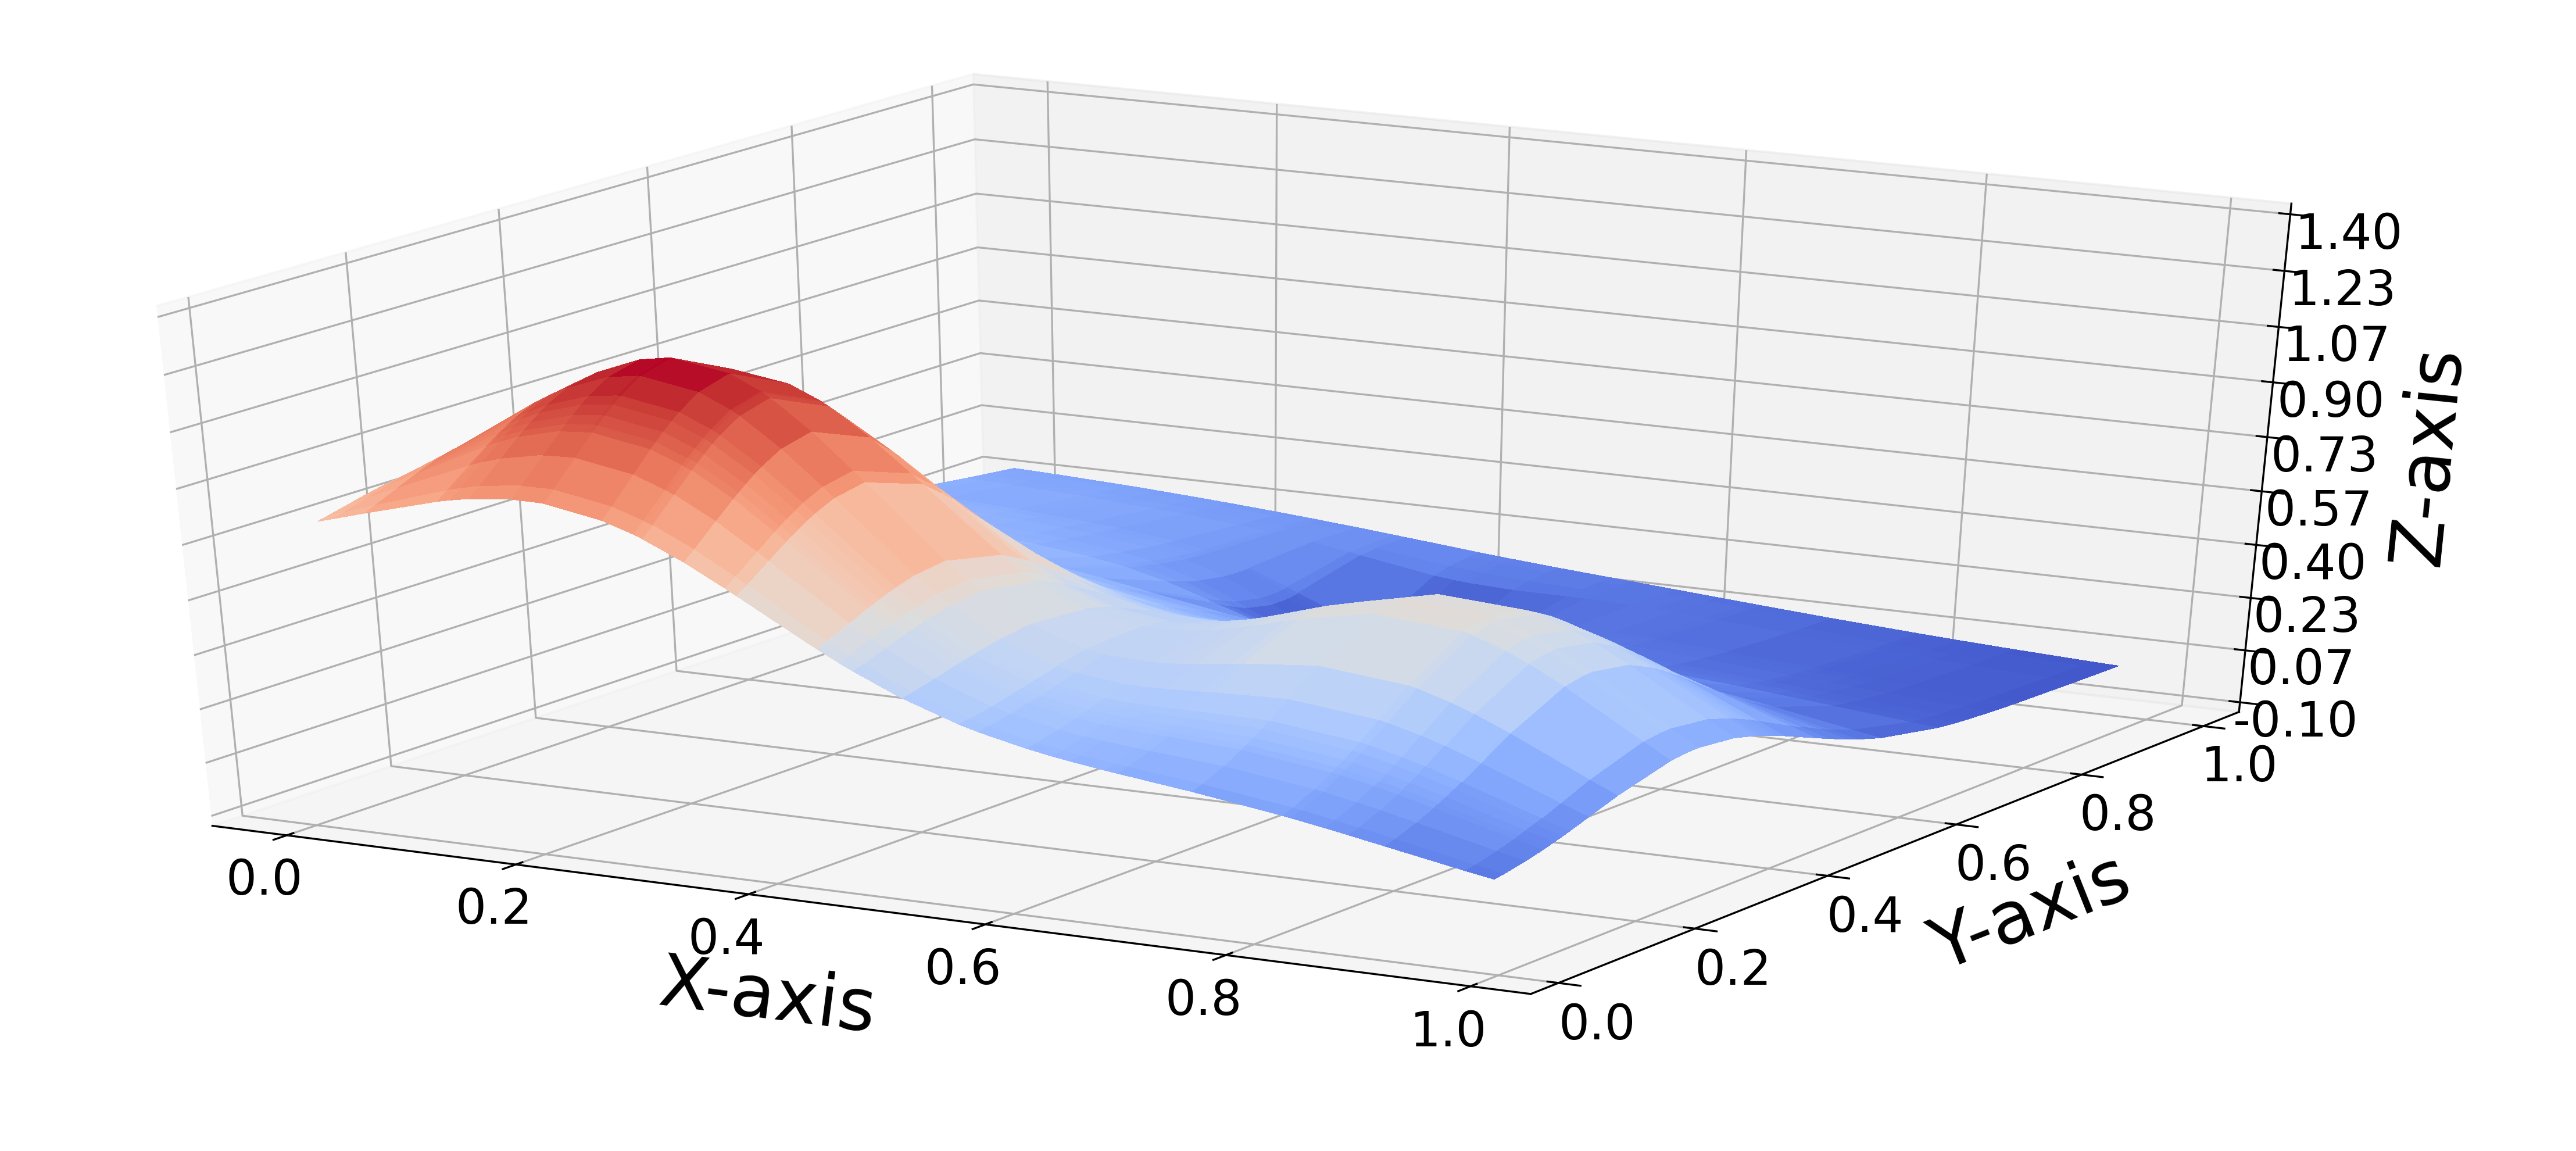
\includegraphics[width=7.9cm]{Figures/Franke_func.png}
\caption{Franke's function}
\label{fig:Frankplt}
\end{figure}

A last term of noise was added to Franke’s function (\ref{eq:Frank}) when generating data for the regression models. The noise was  normal distributed  $N(0,0.1)$.  


\subsubsection{MNIST data set}
This data set contains handwritten digits from zero to nine.
The Tensorflow-Keras API \cite{chollet_keras_2015,martin_abadi_tensorflow_2015} was used to import 60.000 numbers in the training data set and 10.000 numbers in the test data set. Each handwritten digit is a matrix where each number in the matrix represents the color in a grayscale image like in Figure \ref{fig:MNISTnumbers}.
\begin{figure}[!htb]
%\centering
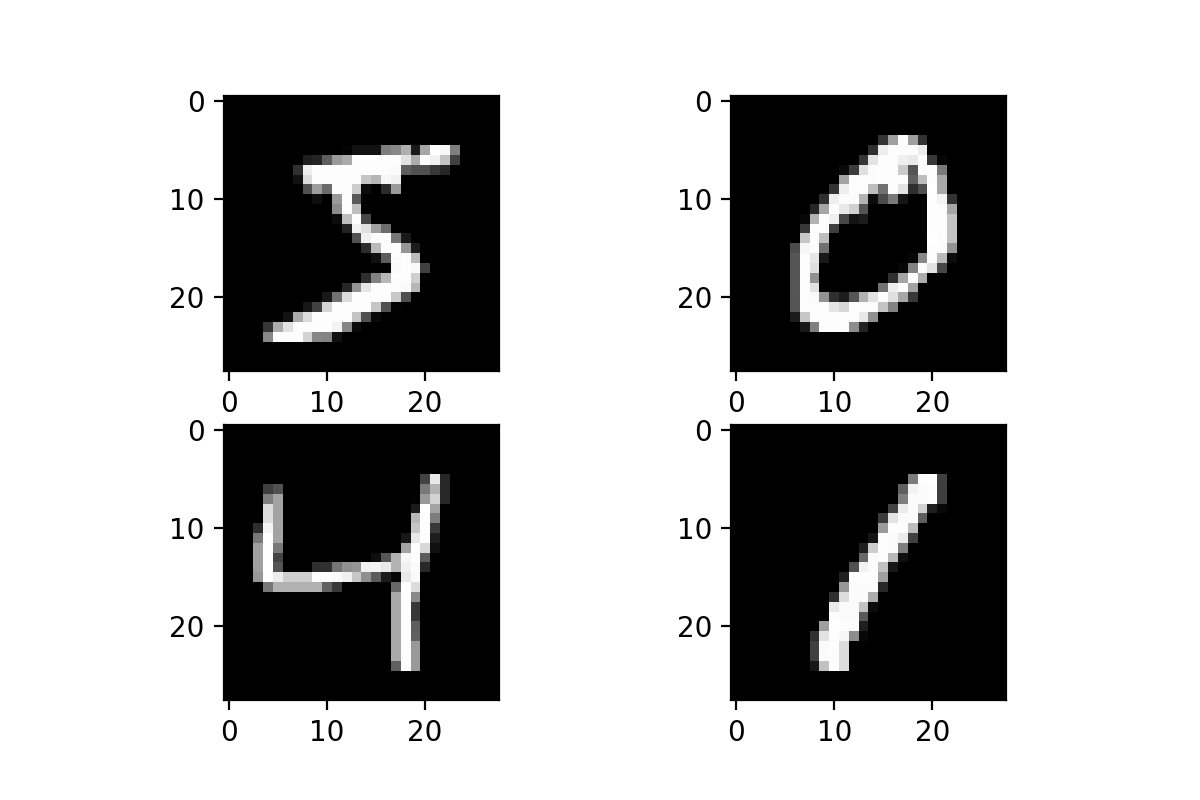
\includegraphics[width=7.9cm]{Figures/MNIST_number.png}
\caption{MNIST examples number}
\label{fig:MNISTnumbers}
\end{figure}
The image was flattened to a $784 \times 1$ array which could be feed into the logistic regression and the neural network. The label of each digit is a number between 0 and 9 and the distribution of the 10 different classes in the training and test set can be seen in Figure \ref{fig:MNISTtrain} and Figure \ref{fig:MNISTtest}


\begin{figure}[!htbp]
%\centering
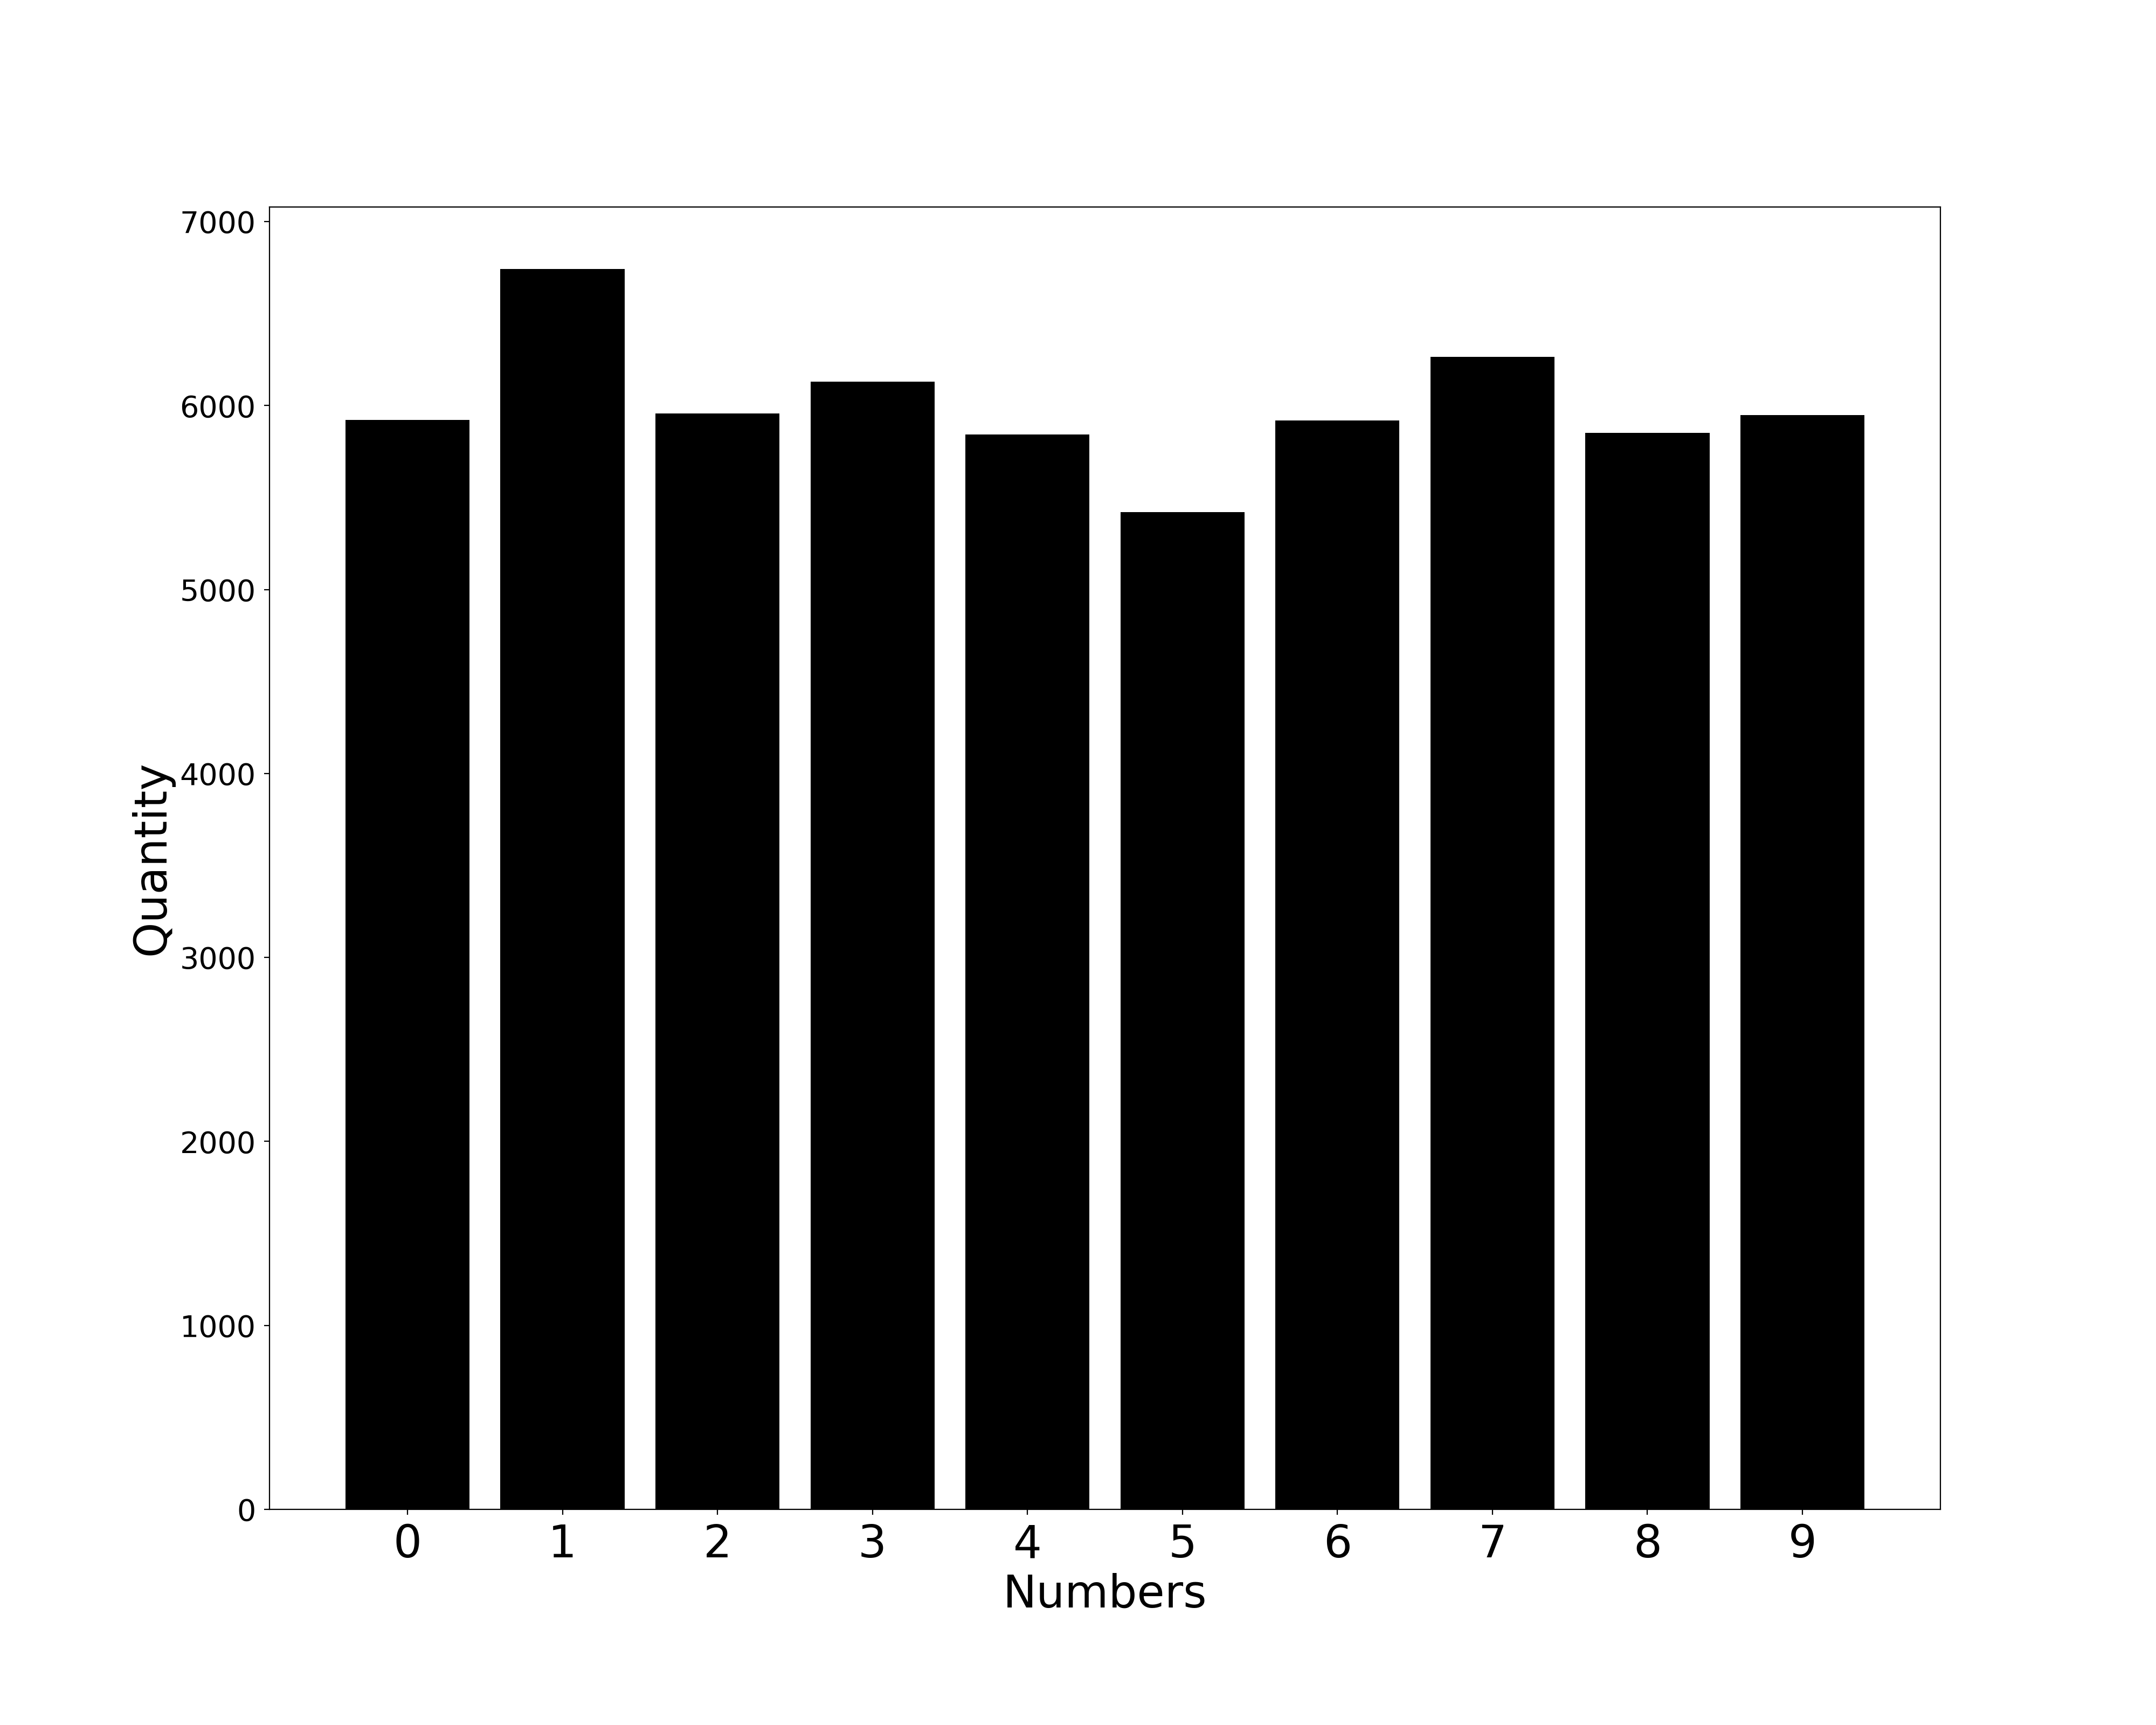
\includegraphics[width=7.9cm]{Figures/MNIST_train_data.png}
\caption{The distribution between classes for the MNIST training data set}
\label{fig:MNISTtrain}
\end{figure}


\begin{figure}[!htbp]
%\centering
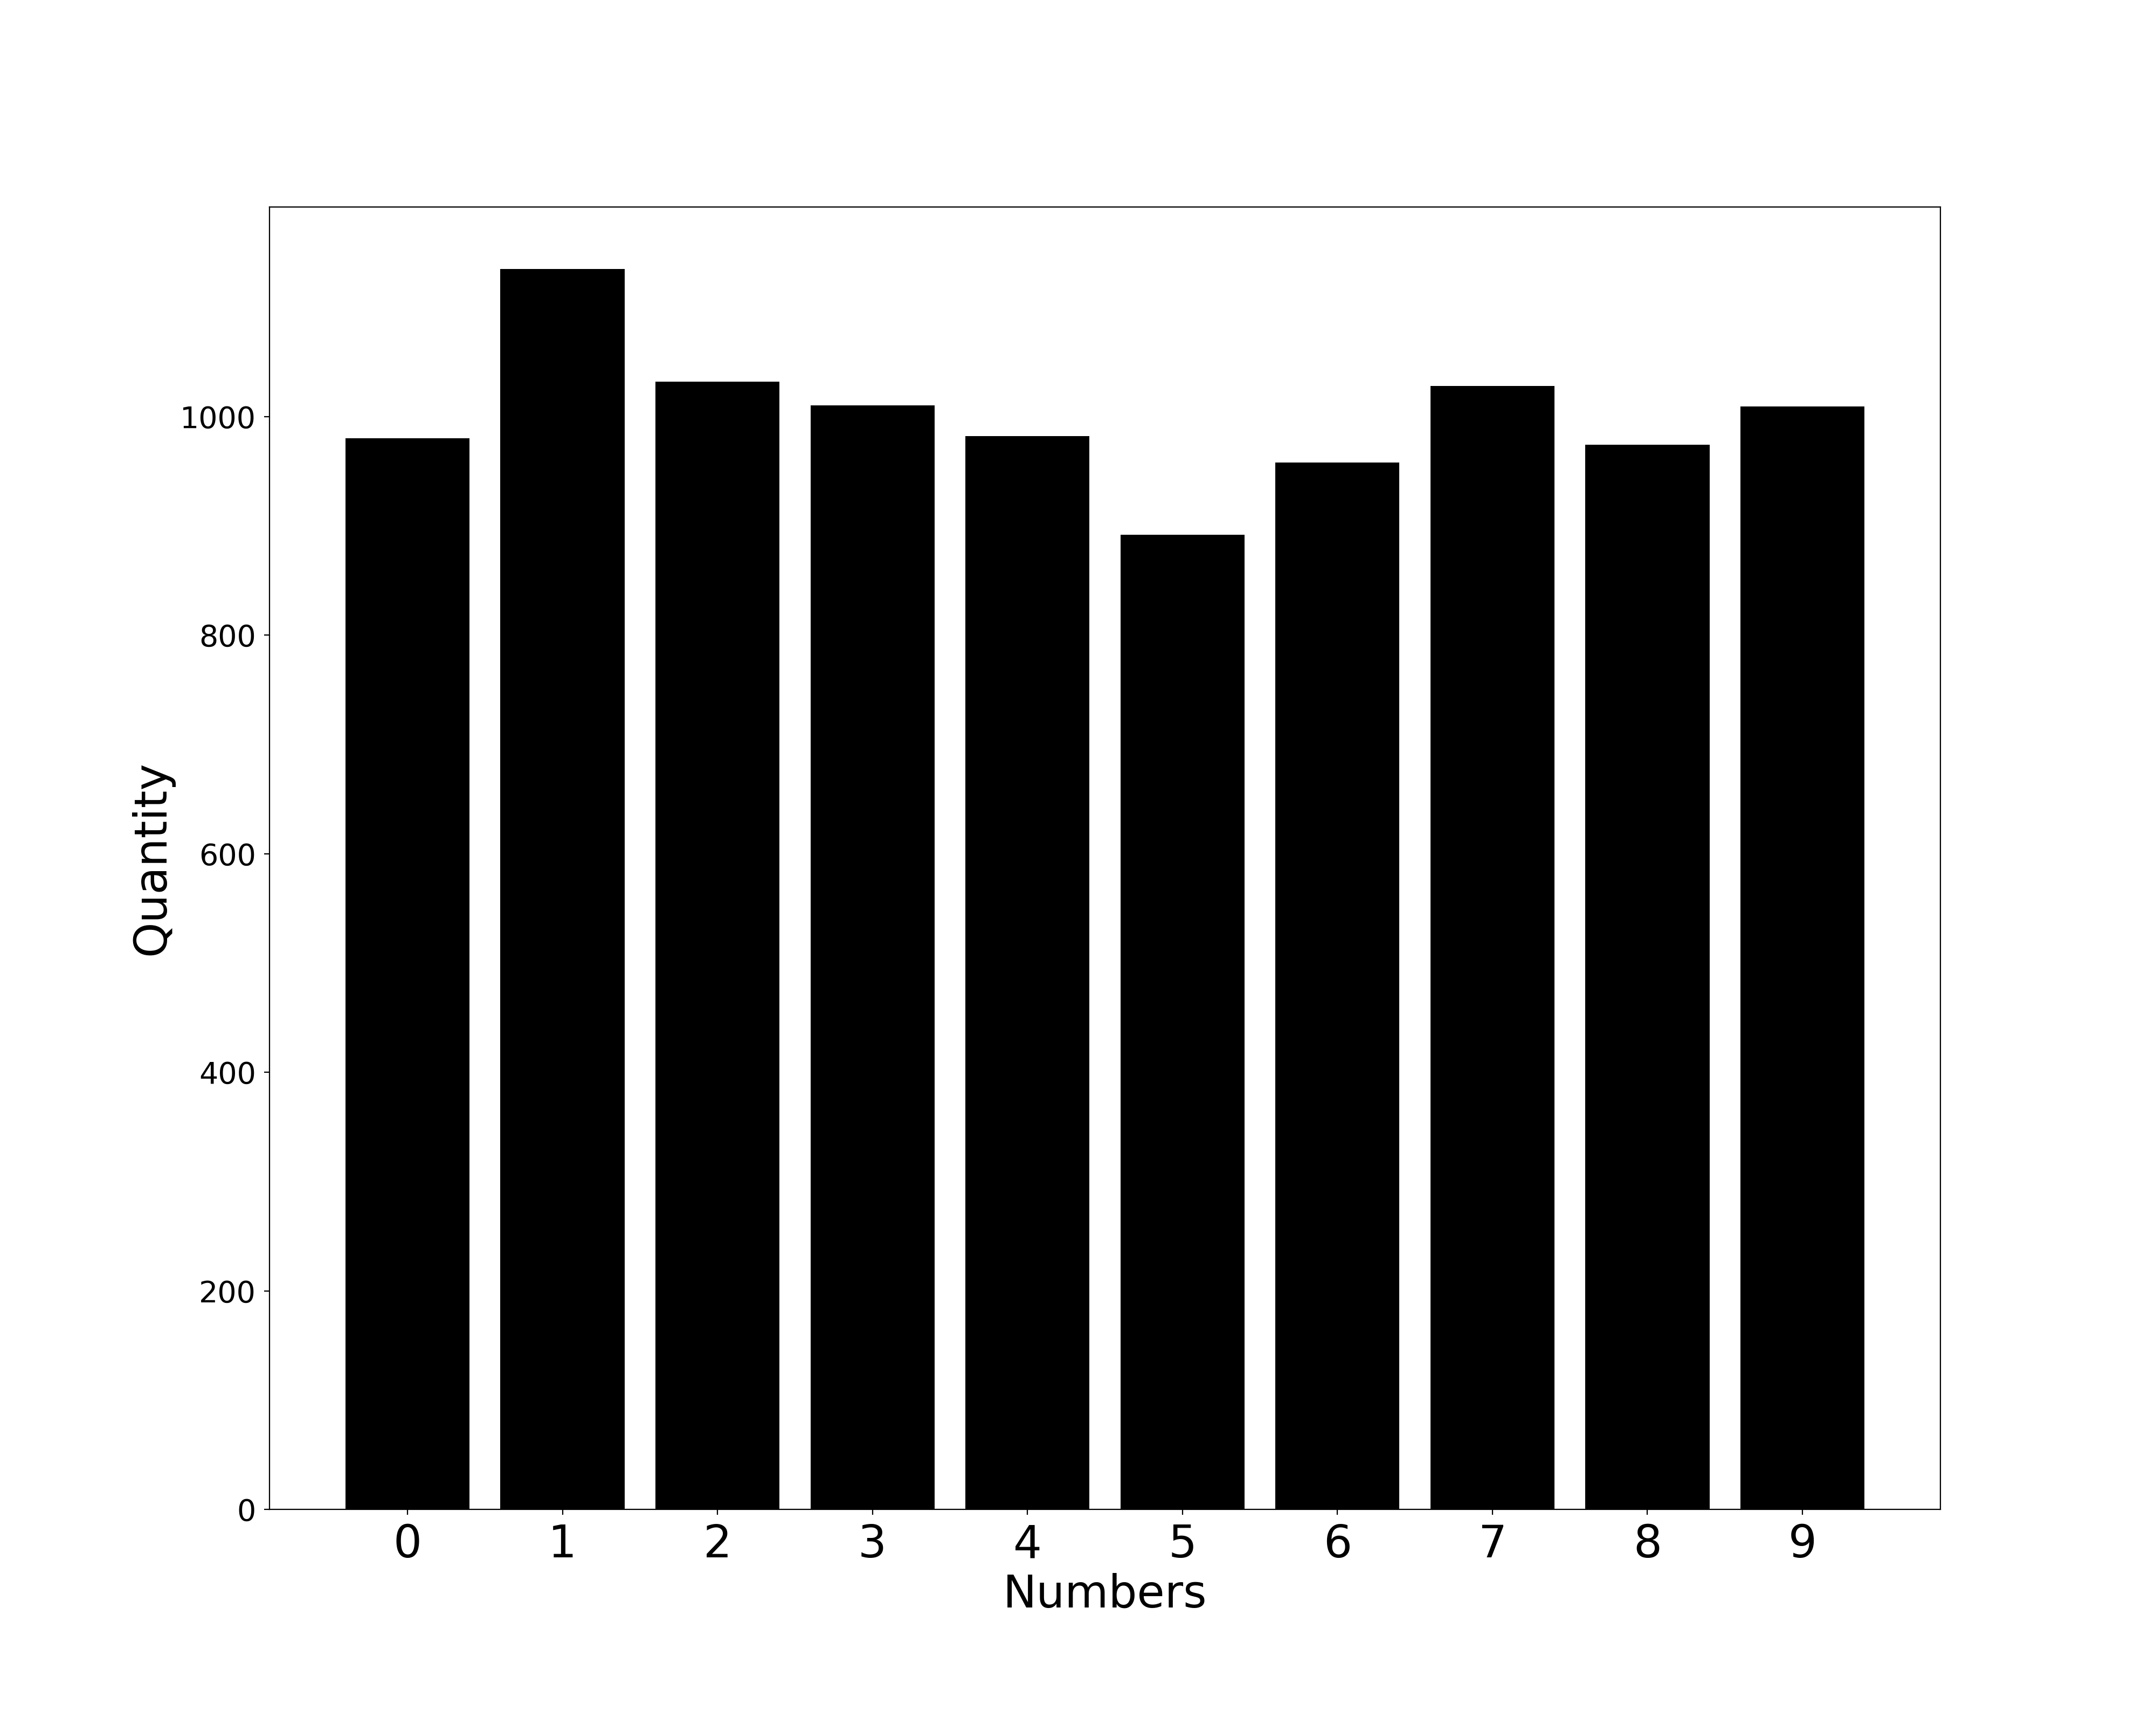
\includegraphics[width=7.9cm]{Figures/MNIST_test_data.png}
\caption{The distribution between classes for the MNIST test data set}
\label{fig:MNISTtest}
\end{figure}


\subsubsection{ECG-data}
The ECG data sets contained a total of 21837 12-lead ECGs from 18885 different patients. All recordings were 10 seconds long and each recording was available as a recording sampled at 500 Hz or downsampled to 100 Hz. In this study, 500Hz was used. The labels in
this data set was the diagnosis given by one or two cardiologists. 24 diagnoses were present in the data set and they were categorized into five broader categories (called super classes) that are used in this study. The five classes are: Conduction Disturbance (CD), Hypertrophy (HP), Myocardial Infarction (MI), Normal class (NORM) and ST/T-change (STTC). A patient could be diagnosed into one or more of these five categories which makes this a multi-label, multi-class classification problem. The data set provider has proposed a test-training-split to make the results comparable across different studies \cite{wagner_ptb-xl_2020}. A stratified fold was used to give the same distribution of diagnoses in the train (see Figure \ref{fig:ECGtrain}) and test (see Figure \ref{fig:ECGtest}) set.

\begin{figure}[!htb]
%\centering
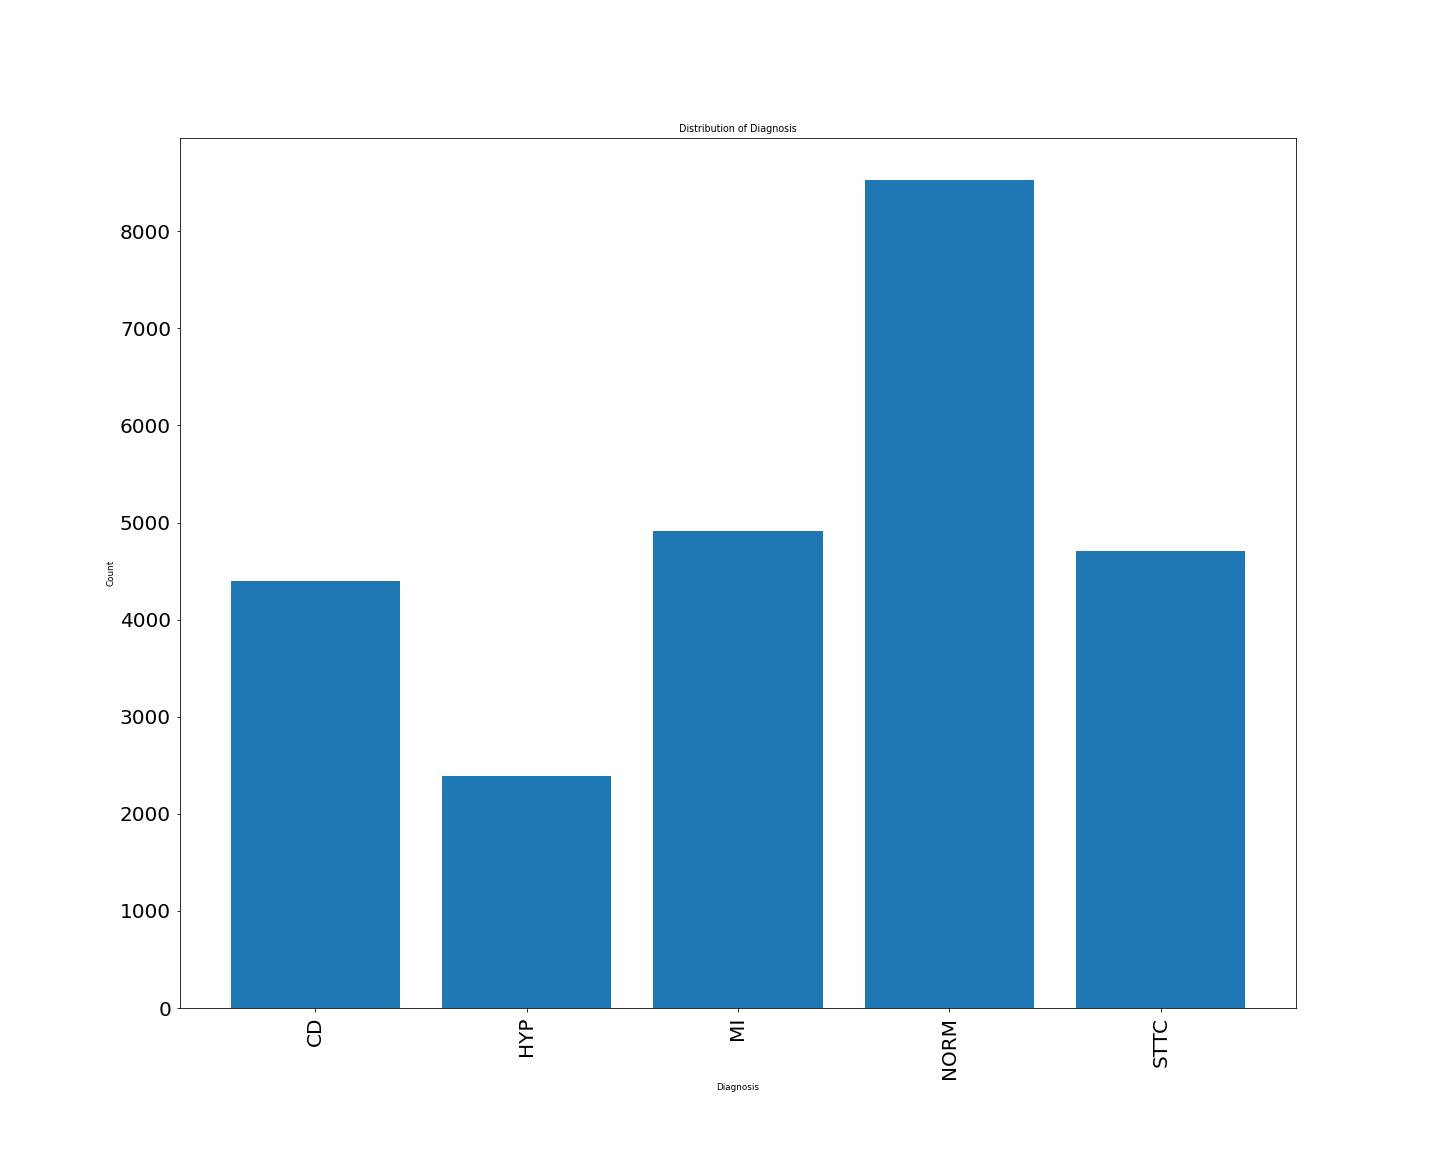
\includegraphics[width=7.9cm]{Figures/distribution_training.png}
\caption{The distribution between classes for the PTB-XL ECG training data set}
\label{fig:ECGtrain}
\end{figure}

\begin{figure}[!htb]
%\centering
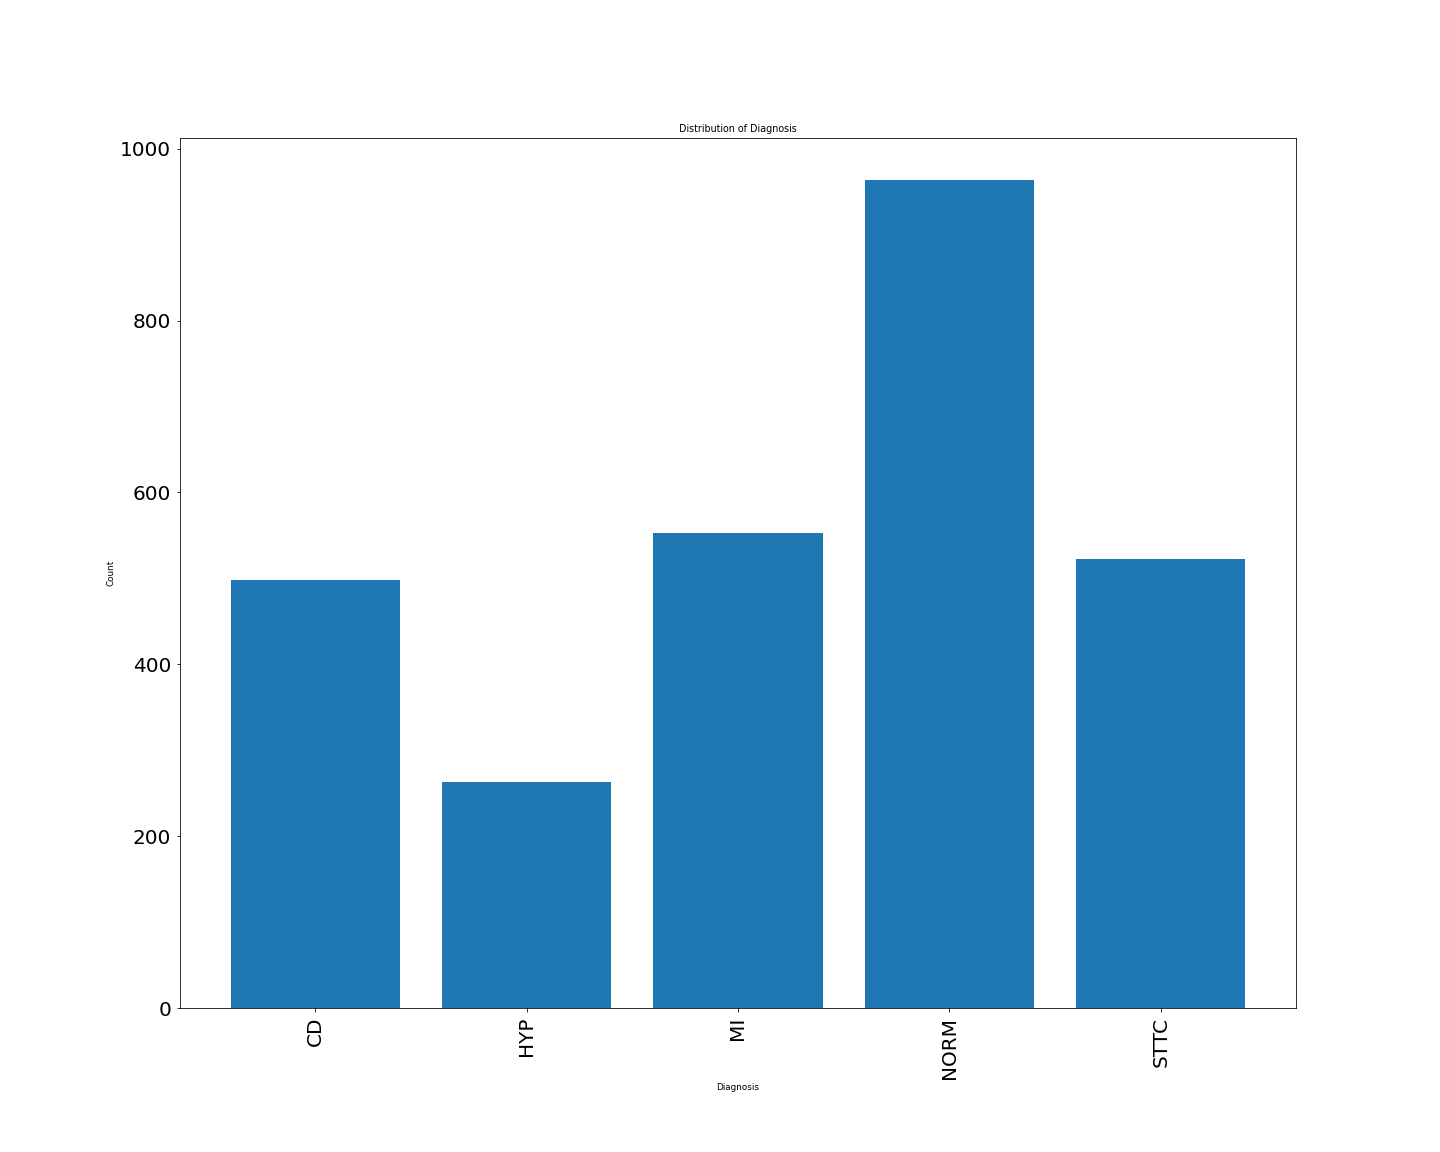
\includegraphics[width=7.9cm]{Figures/distribution_test.png}
\caption{The distribution between classes for the PTB-XL ECG test data set}
\label{fig:ECGtest}
\end{figure}

To be able to use the ECG data as input to a classifier, such as a neural network or a logistic regression model, the data was processed by extracting features instead of using the whole waveform as an input. This was done by developing a new Python package, ECG-featurizer\cite{bjorn-jostein_singstad_ecg-featurizer_nodate}, based on NeuroKit2 \cite{makowski_neurokit2_2020} and the Waveform database (WFDB) package. The ECG-featurizer extracted 112 features from each ECG-recording.


\subsection{Regression algorithms}
\subsubsection{Linear regression with SGD optimizer}
As a starting point for the regression analysis, the OLS and Ridge regression models developed in \cite{bjorn-jostein_singstad_using_nodate} was trained once again. First, the polynomial degree of the OLS model was found using a search from polynomial degree one to 20 using the mean of a 10-fold cross-validated R2-score.
The best polynomial degree from the OLS model was used as the degree in the Ridge model and a search through $\lambda$-values from $0.000001$ to $1000$ increasing with a factor of $10$ for each step. The best $\lambda$-values were selected based on the mean of a 10-fold cross-validated R2-score.

Further, the design matrix in the OLS-algorithm was replaced with a stochastic gradient descent (SGD) optimization algorithm and employed on the data generated by Franke's function. A grid search was performed and a 3-fold cross-validated accuracy score was used to find the optimal parameters of the learning rate ($\gamma)$, batch size, learning rate reduction and the number of epochs.

\subsubsection{Regression using neural network}
A neural network with linear activation in the final layer was developed. The linear activation in the final layer was necessary for doing regression. The optimal parameters were found doing two grid search. The first grid search was searching for the optimal learning rate, number of hidden layers, number of hidden units (neurons), activation functions in the hidden layer. The second grid search was searching for the optimal number of epochs, batch size, weight initialization, and bias initialization. The optimal parameters found in the grid search one were used in grid search two. 3-fold cross-validation was used during both grid search and the best mean R2-score over the three folds was used as the measure for selecting parameters.

\subsection{Classification}
\subsubsection{Classifying MNIST data}

The neural network used to classify MNIST data used Softmax activation (eq \ref{eq:softmax})in the final layer. This is typical for a classification problem were each input data only have one label (not multi-label).
\begin{equation}
softmax(x)_i = \frac{exp(x_i)}{\sum_{j}^{ }exp(x_j))}
\label{eq:softmax}
\end{equation}
The optimal parameters of the neural network were found using graduate student descent method. The model with the optimal parameters were validated using 5-fold cross validation and tested on a unused test set.

In addition, a Logistic Regression algorithm was developed, tested and compared with the neural network.

\subsubsection{Classifying PTB-XL ECG data}
Since the PTB-XL ECG data were a multi-class, multi-label classification problem the neural network had to use a Sigmoid activation(eq \ref{eq:sigmoid}) in the final layer
\begin{equation}
h_ \theta (x) =  \frac{\mathrm{1} }{\mathrm{1} + e^-\theta^Tx}
    \label{eq:sigmoid}
\end{equation}
The hyperparameters were optimized using Bayesian Tuner \cite{omalley_keras_2019}. The 1st validation fold of a 10-fold stratified cross-validation was used for the optimization to speed up the search. 

The ECG classification and thus the prediction threshold had to be set. The threshold was optimized when the model was successfully trained. This was done by running the classifier on the test set and receiving a score between 0 and 1 for each of the classes. A search through thresholds was done using a 5-bit long array of ones and that got multiplied with values from 0 to 1 with a step size of 0.01 which resulted in 100 different thresholds. The accuracy score for the training data was evaluated for each threshold. The best threshold was used as an initial guess for the Nelder-Mead downhill simplex method \cite{nelder_simplex_1965, virtanen_scipy_2020}. This algorithm optimized the threshold for each class individually. The Nelder-Mead downhill simplex method is used to find the local minimum of a function using the function itself and an initial guess of the variable of the function. The 5-element long array was optimized using the negative of the accuracy score and thus resulted in the best possible accuracy score for the given model.

Also, a Logistic Regression algorithm was developed, tested and compared with the neural network.


\section{Results}
\subsection{Regression}
\subsubsection{OLS}
The best polynomial degree of the OLS algorithm is based on the mean of a 10-fold cross-validated R2-score. Polynomial degrees from 1 to 20 were tested and a degree of 9 turned out to be best.
\subsubsection{Ridge}
The polynomial degree of 9 was used in the Ridge model and $\labdas$ from $0.000001$ to $1000$ were tested and selected using the mean of a 10-fold cross-validated R2-score. The best $\labdas$ turned out to be $0.1$

Both the OLS and the Ridge model were then cross validated using their optimized parameter. The cross validated R2-score for OLS was: median$=0.831 \pm0.019$SD and median$=0.015 \pm0.002$SD for MSE. The cross validated R2-score for Ridge was: median$=0.830 \pm0.016$SD.\newline
MSE Ridge:$=0.015 \pm0.001$SD for MSE. The results are also presented in figure \ref{fig:OLS_ridge}.
\begin{figure}[htbp!]
%\centering
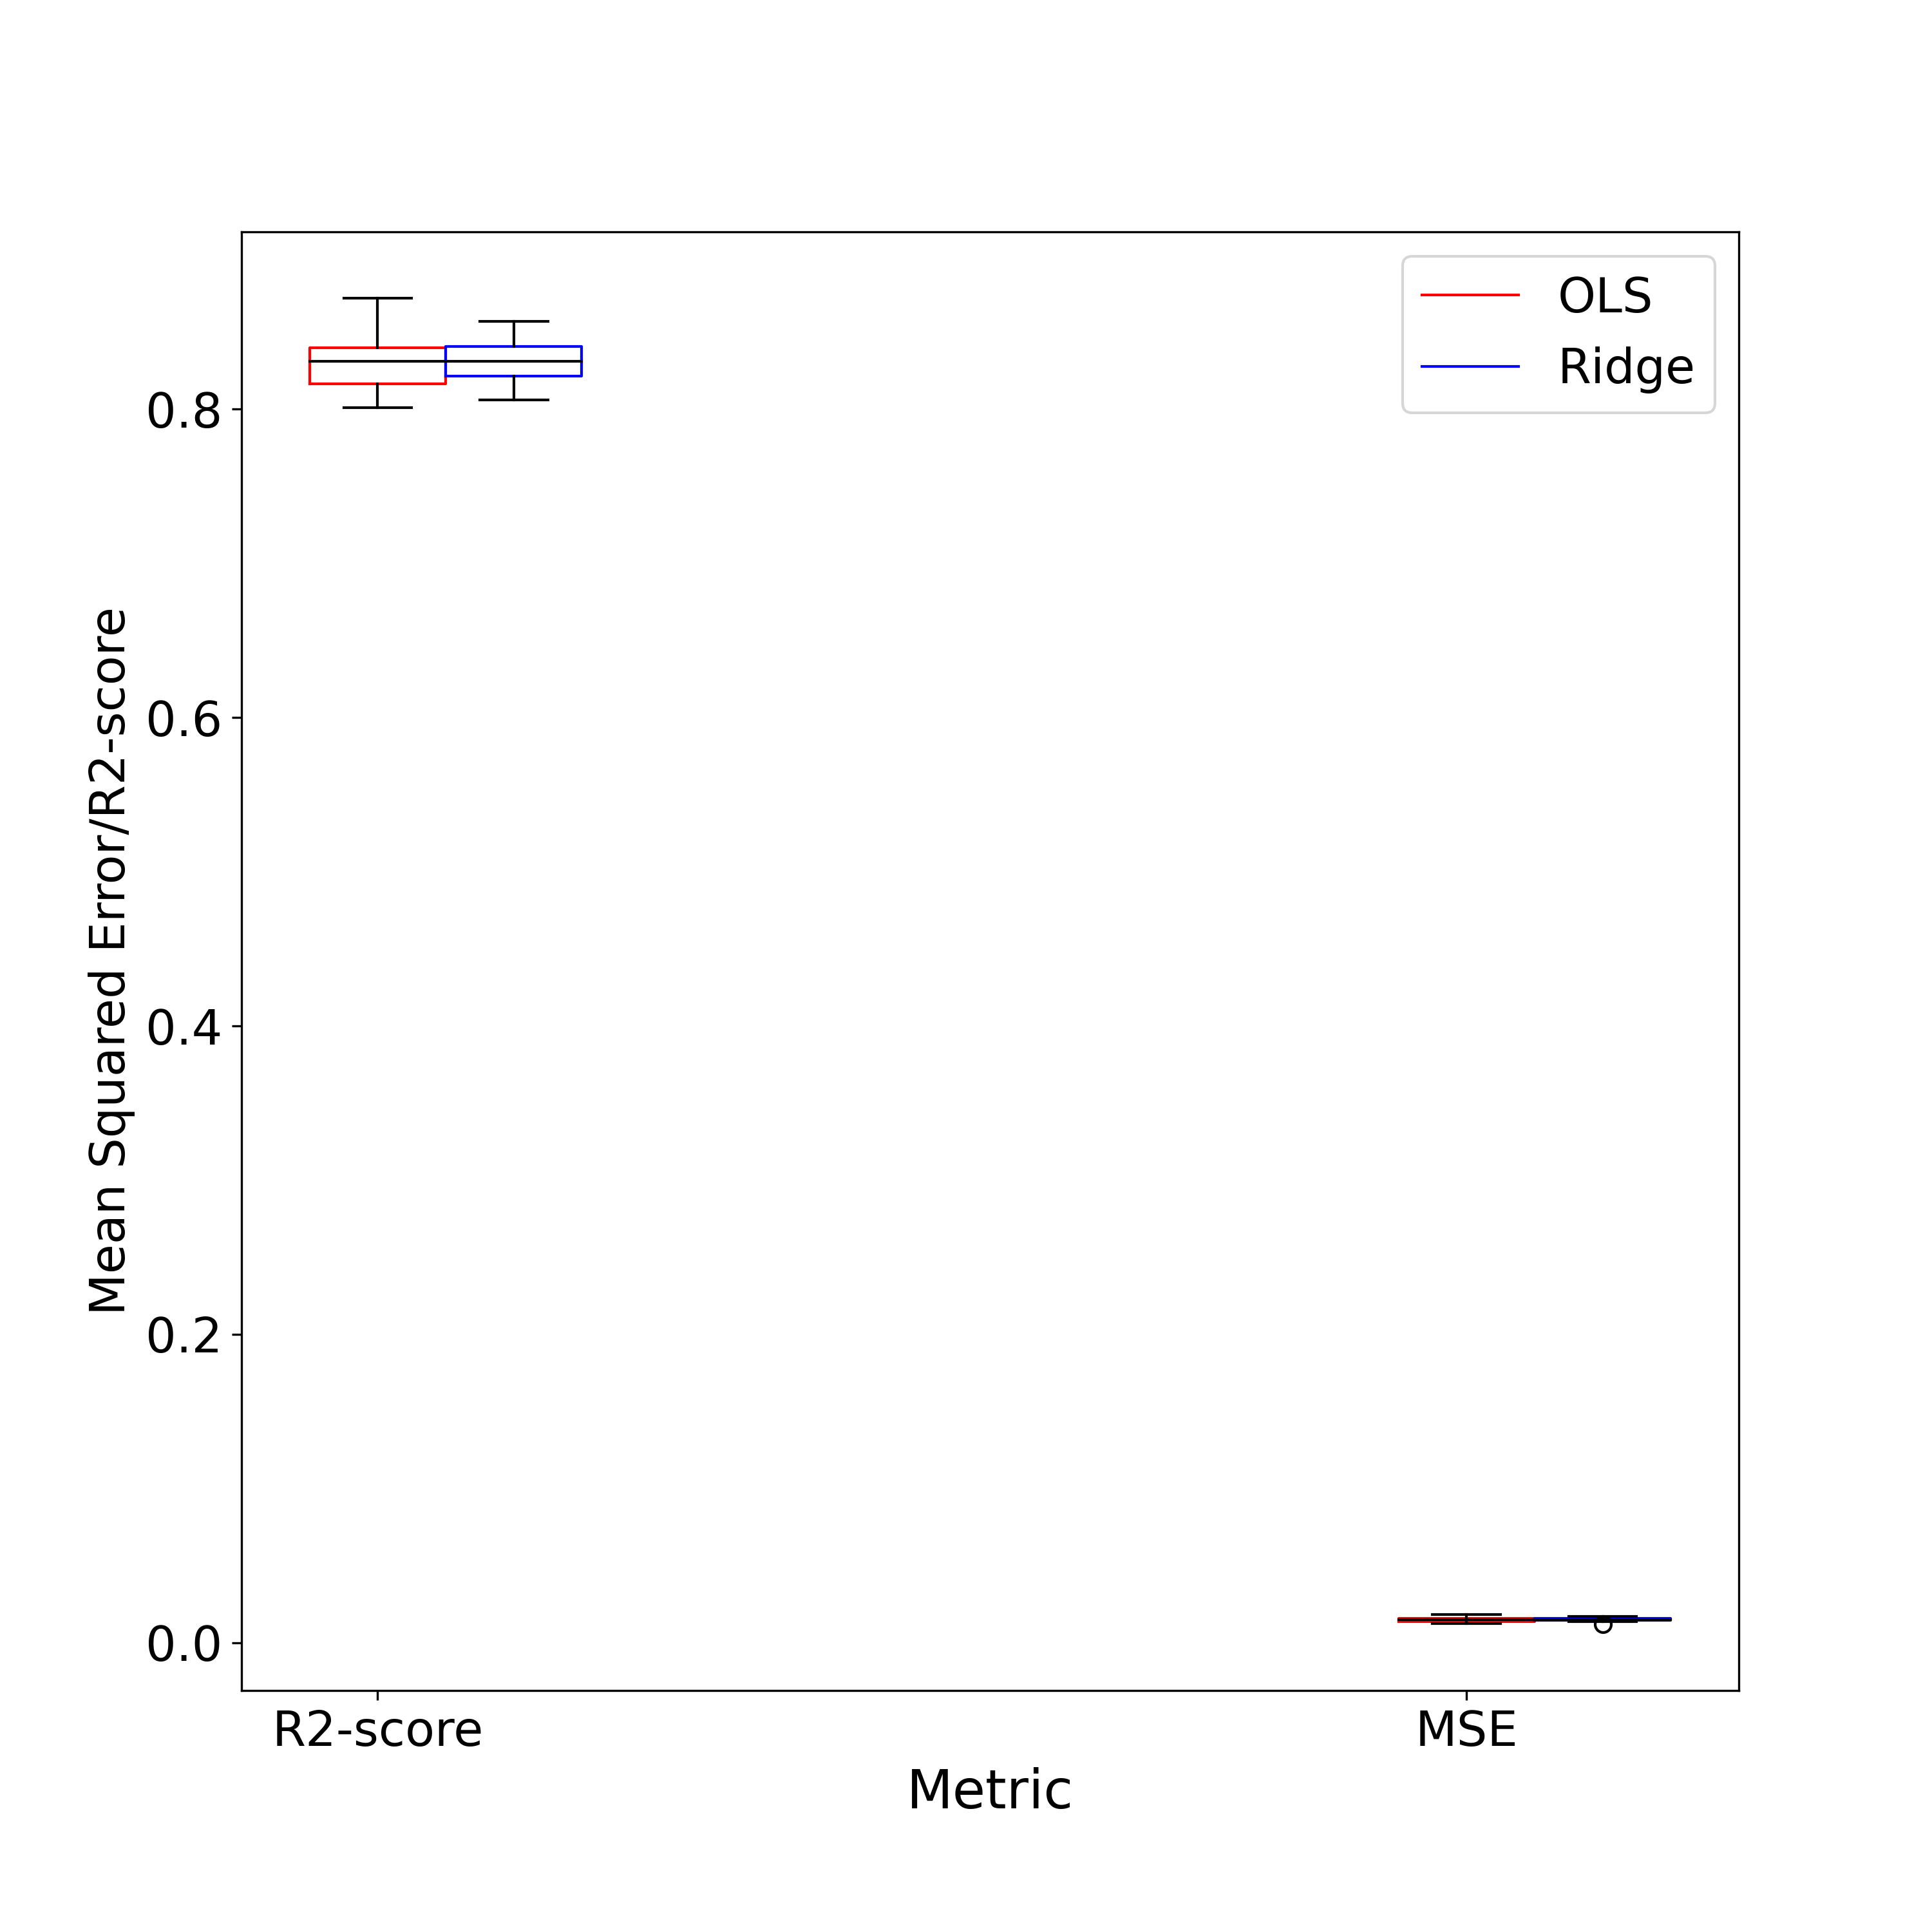
\includegraphics[width=7.9cm]{Figures/boxplot_OLS_ridge.png}
\caption{The red boxes shows the cross validated R2-score and MSE achieved by the OLS algorithm using a polynomial degree$=9$. The blue boxes shows the cross validated R2-score and MSE achieved by the Ridge algorithm using a polynomial degree$=9$ and a $\lambda = 0.1$}
\label{fig:OLS_ridge}
\end{figure}

\subsubsection{SGD OLS}
The SGD OLS model selection were done using 3 fold cross validation. The parameters that were search through using grid search are shown in table \ref{tab:gridsearch_sgd}

\vspace{-4 mm}
\begin{table}[!htpb]
\vspace{4 mm}
\caption{\label{tab:gridsearch_sgd} Grid search parameters used to optimize OLS SGD}
\centerline{\begin{tabular}{lr} \hline\hline
Parameter                       & Values         \\ \hline
Learning rate ($\gamma$)   &  $0.01, 0.001, 0.0001$  \\
Batch size             & $30,50,70$               \\ 
Learning rate reduction          & $10^{-5}, 10^{-3}, 10^{-1}$                \\  
Epochs & $5,10,15$ \\\hline\hline
\end{tabular}}

\end{table}

The results did not seem to be right and figure \ref{fig:appendix_sdg} in appendix shows the OLS SDG together with Ridge and OLS.


\subsubsection{neural network Regression}
Hyperparameters for the neural network were found doing a grid search on a small subset of the data generated by Franke's function. The resampling function from Scikit-learn \cite{pedregosa_scikit-learn_2011} was used to pick $200$ random samples from the total $1600$ data points. The parameter optimization was divided into two grid searches. The 1st grid search was done using the parameters in table \ref{tab:gridsearch_nn_reg}.


\vspace{-4 mm}
\begin{table}[!htpb]
\vspace{4 mm}
\caption{\label{tab:gridsearch_nn_reg}  Grid search number 1. These parameters were optimized using grid search on the neural network employed on a subset of the total data set generated by Franke's function.}

\centerline{\begin{tabular}{lr} \hline\hline
Parameter                       & Values                                \\ \hline
Learning rate                   &  $0.1,0.001,0.00001$                  \\                      
Hidden layers                   & $1,4,7$                               \\
Hidden units                    &  $50,100,150$                         \\
Activation in hidden layers     & ReLU, Sigmoid, SeLU                   \\\hline\hline
\end{tabular}}
\end{table}
The best parameters found in grid search 1 was then used in grid search 2. The parameters optimized in grid search 2 is shown in table \ref{tab:gridsearch_nn_reg2}.
\newline
\vspace{-4 mm}
\begin{table}[!htpb]
\vspace{4 mm}
\caption{\label{tab:gridsearch_nn_reg2} Grid search number 2. These parameters were optimized using grid search on the neural network employed on a subset of the total data set generated by Franke's function.}

\centerline{\begin{tabular}{lr} \hline\hline
Parameter                       & Values    \\ \hline
Epoch                   &  $10,50,100$  \\
Batch size                      & $10,50,100$     \\              
Bias initialization                   &  zeros, RandomNormal, \\                                            &    RandomUniform     \\
Weight initialization                    & zeros, RandomNormal,\\                                           &  RandomUniform   \\\hline\hline
\end{tabular}}
\end{table}

A 3-fold cross-validation was used during grid search and the best mean of the R2-score computed for each fold was used as the measure for selecting the best parameters. 

Finally, the optimized parameters were used in the model when performing a 10-fold cross-validation on the whole data set. The neural network achieved a cross-validated R2-score of  median$=0.857\pm 0.021SD$ and a cross-validated MSE of median$=0.012\pm 0.001SD$ 


\subsection{Neural network for classification}
\subsubsection{Classification of MNIST-data using neural network}
The optimal parameters of the neural network used to classify the MNIST data were found using graduate student descent. The model was then validated by doing 5-fold cross-validation and achieved an R2-score of: median=$0.851 \pm 0.002SD$. On the test set, the model performed an accuracy score of $0.8665$. A confusion matrix for the model can be seen in figure \ref{fig:NN_mnist_confmatrix}.

\begin{figure}[htbp!]
%\centering
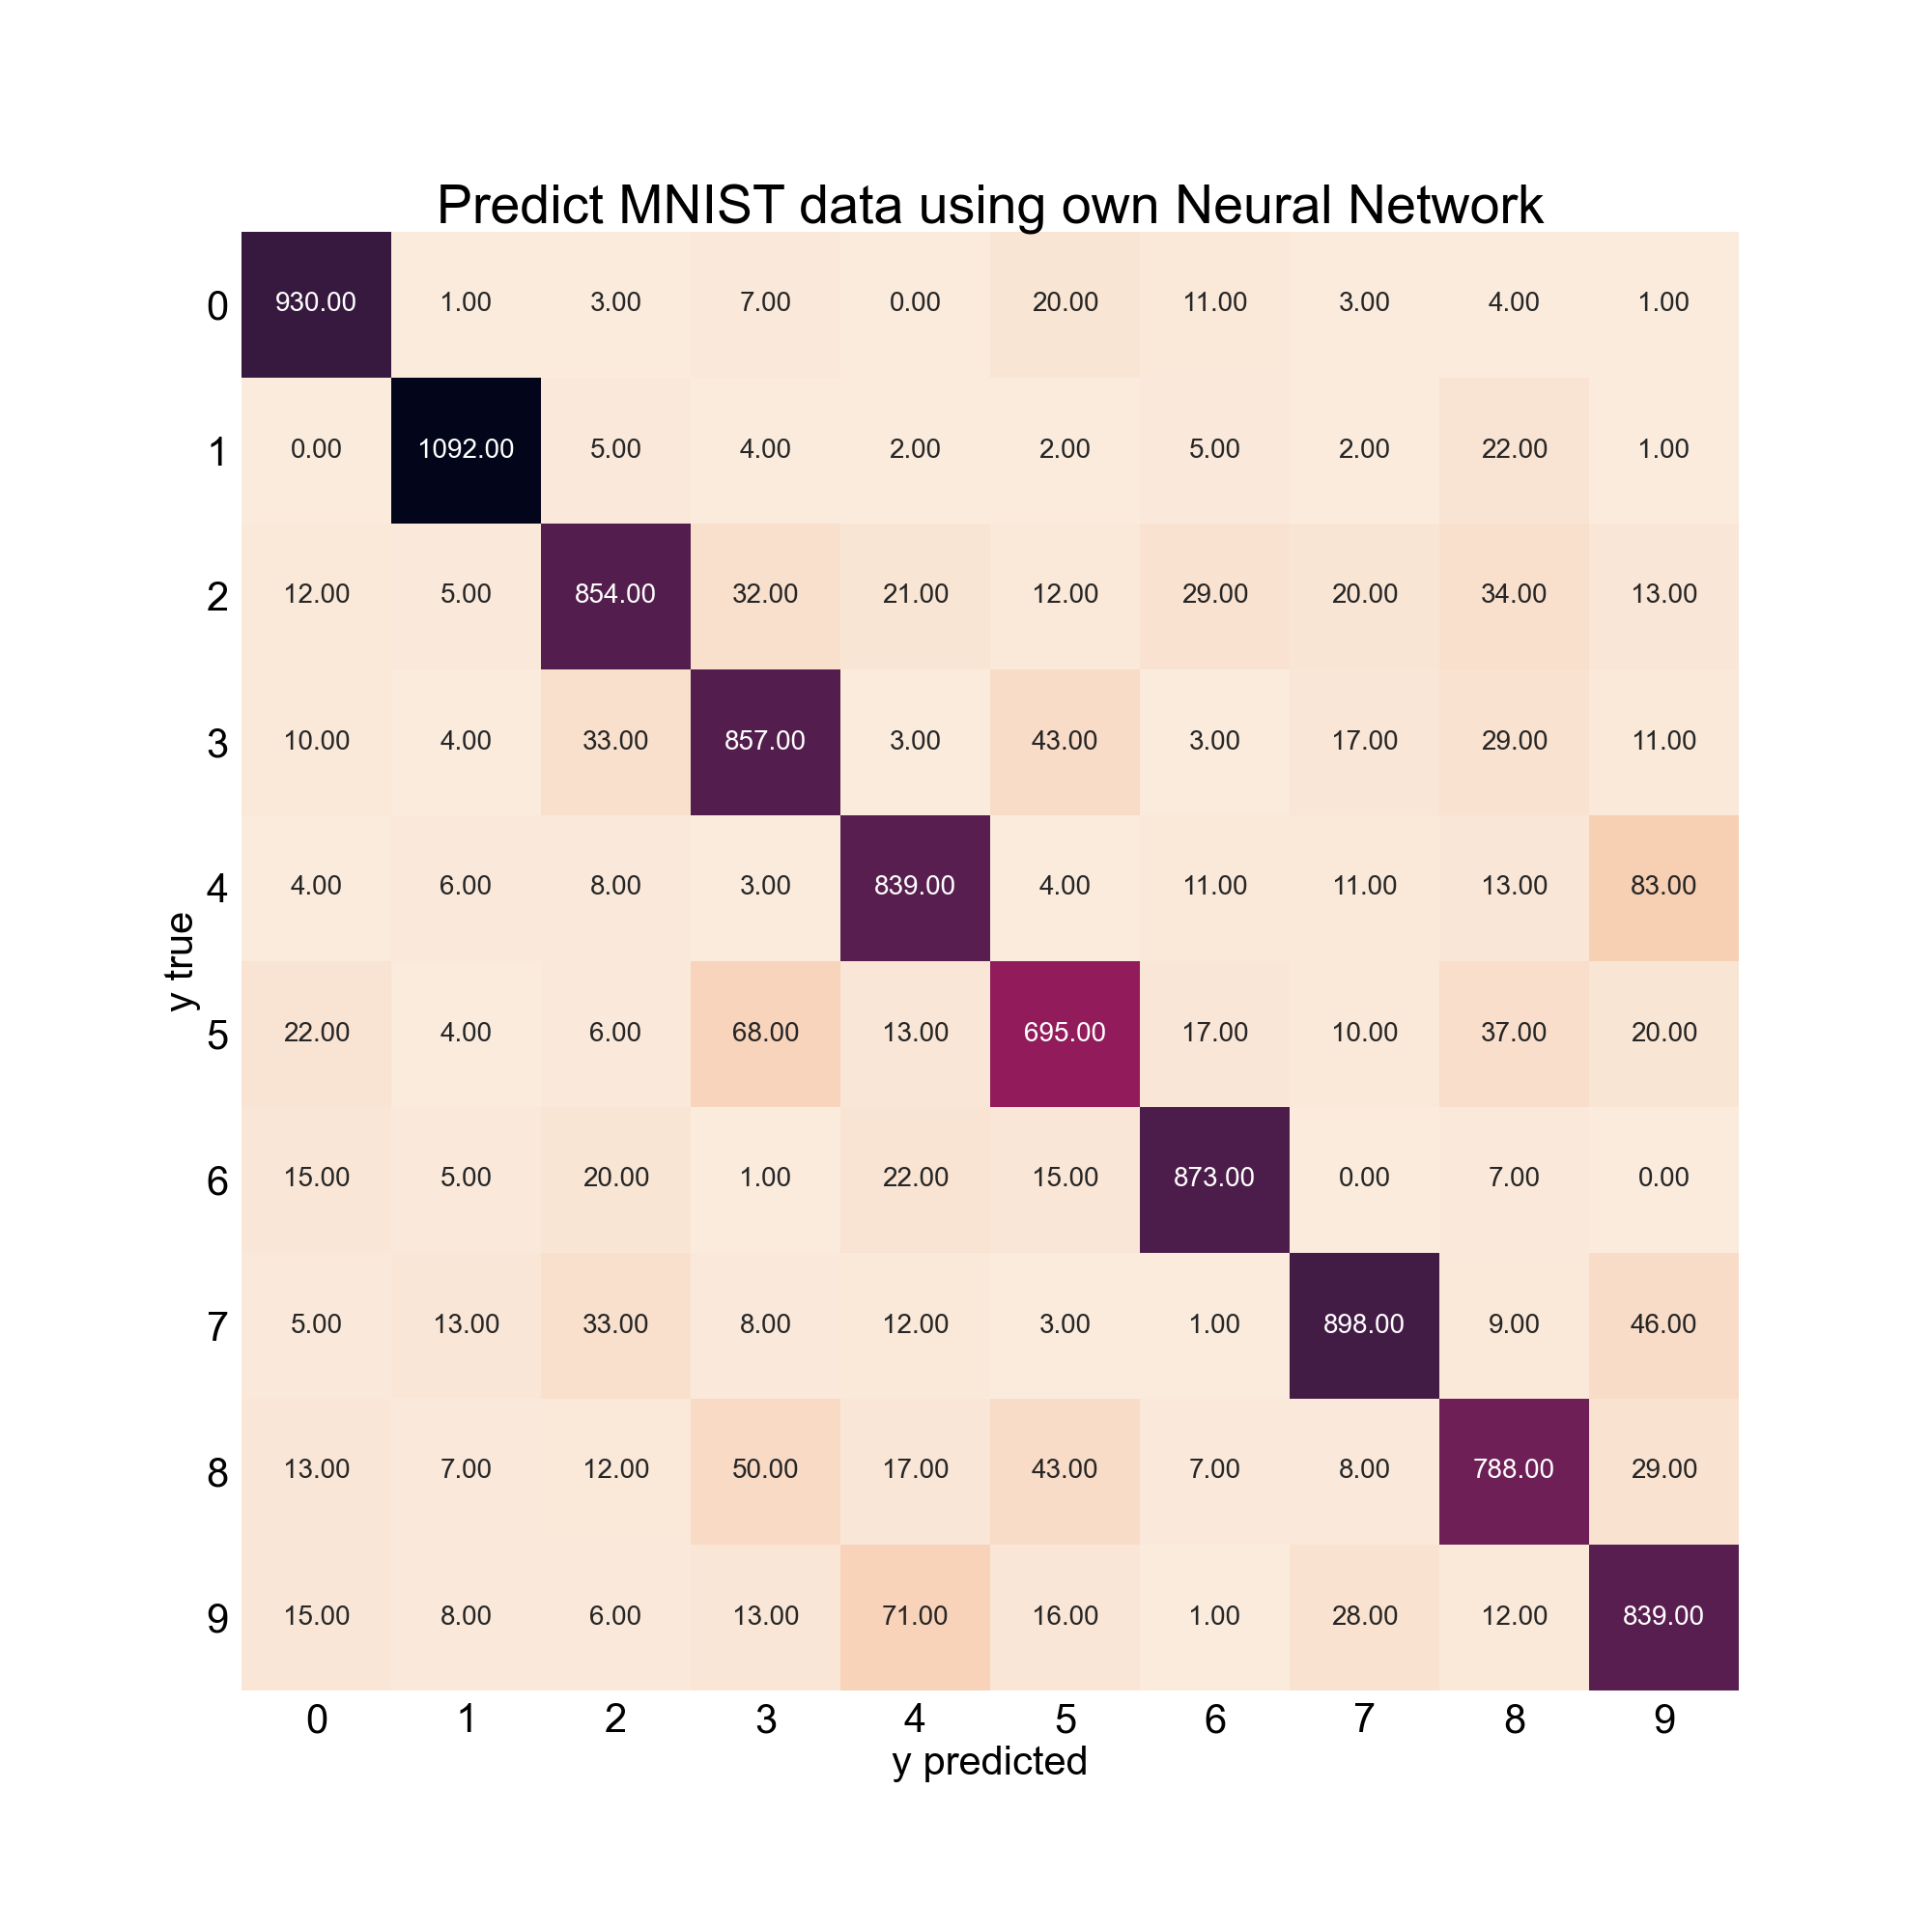
\includegraphics[width=7.9cm]{Figures/MNIST_confMatrix_ownNN.png}
\caption{Confusion matrix - neural network performing prediction on test set of MNIST data}
\label{fig:NN_mnist_confmatrix}
\end{figure}



\subsubsection{Classification of ECG data using neural network}
The ECG-featurizer \cite{bjorn-jostein_singstad_ecg-featurizer_nodate} managed to analyze 19609 out of 19635 of training data and 2203 out of 2203 of test data. The remaining 26 training data were taken out of the data set. Some NaN-values were also present in the training set. These were replaced by the mean of all the other values in the same category. 
Google Colab was used to do Bayesian optimization. Validation accuracy loss was used as the target to optimize the model.

\vspace{-4 mm}
\begin{table}[!htpb]
\vspace{4 mm}
\centerline{\begin{tabular}{lr} \hline\hline
Parameter                       & Values         \\ \hline
Learning rate   &  $1^{-5}, 1^{-4}, 1^{-3}, 0.01, 0.1$  \\
Batch size             & $10,20,30,...,100$               \\ 
Hidden layers           & $1,2,3,...,11$                \\  
Activation in hidden layers & ReLU, eLU, SeLU \\\hline\hline
\end{tabular}}
\caption{\label{tab:challenge_validation} Parameters used in the Bayesian optimization of the neural network used for classification of the PTB-XL ECG data.}
\end{table}

The accuracy score achieved on the test set proposed by the publisher of the PTB-XL ECG data was $0.415$
The conf matrix looks like this:

\subsection{Logistic regression}
\subsubsection{Classification of MNIST-data}
The logistic regression model trained for 100 iterations on the MNIST data set achieved a accuracy score of 0.93 on the test set. The performance on the test set is also shown in figure \ref{fig:confmatrixlog_MNIST} as a confusion matrix. 
\begin{figure}[htbp!]
%\centering
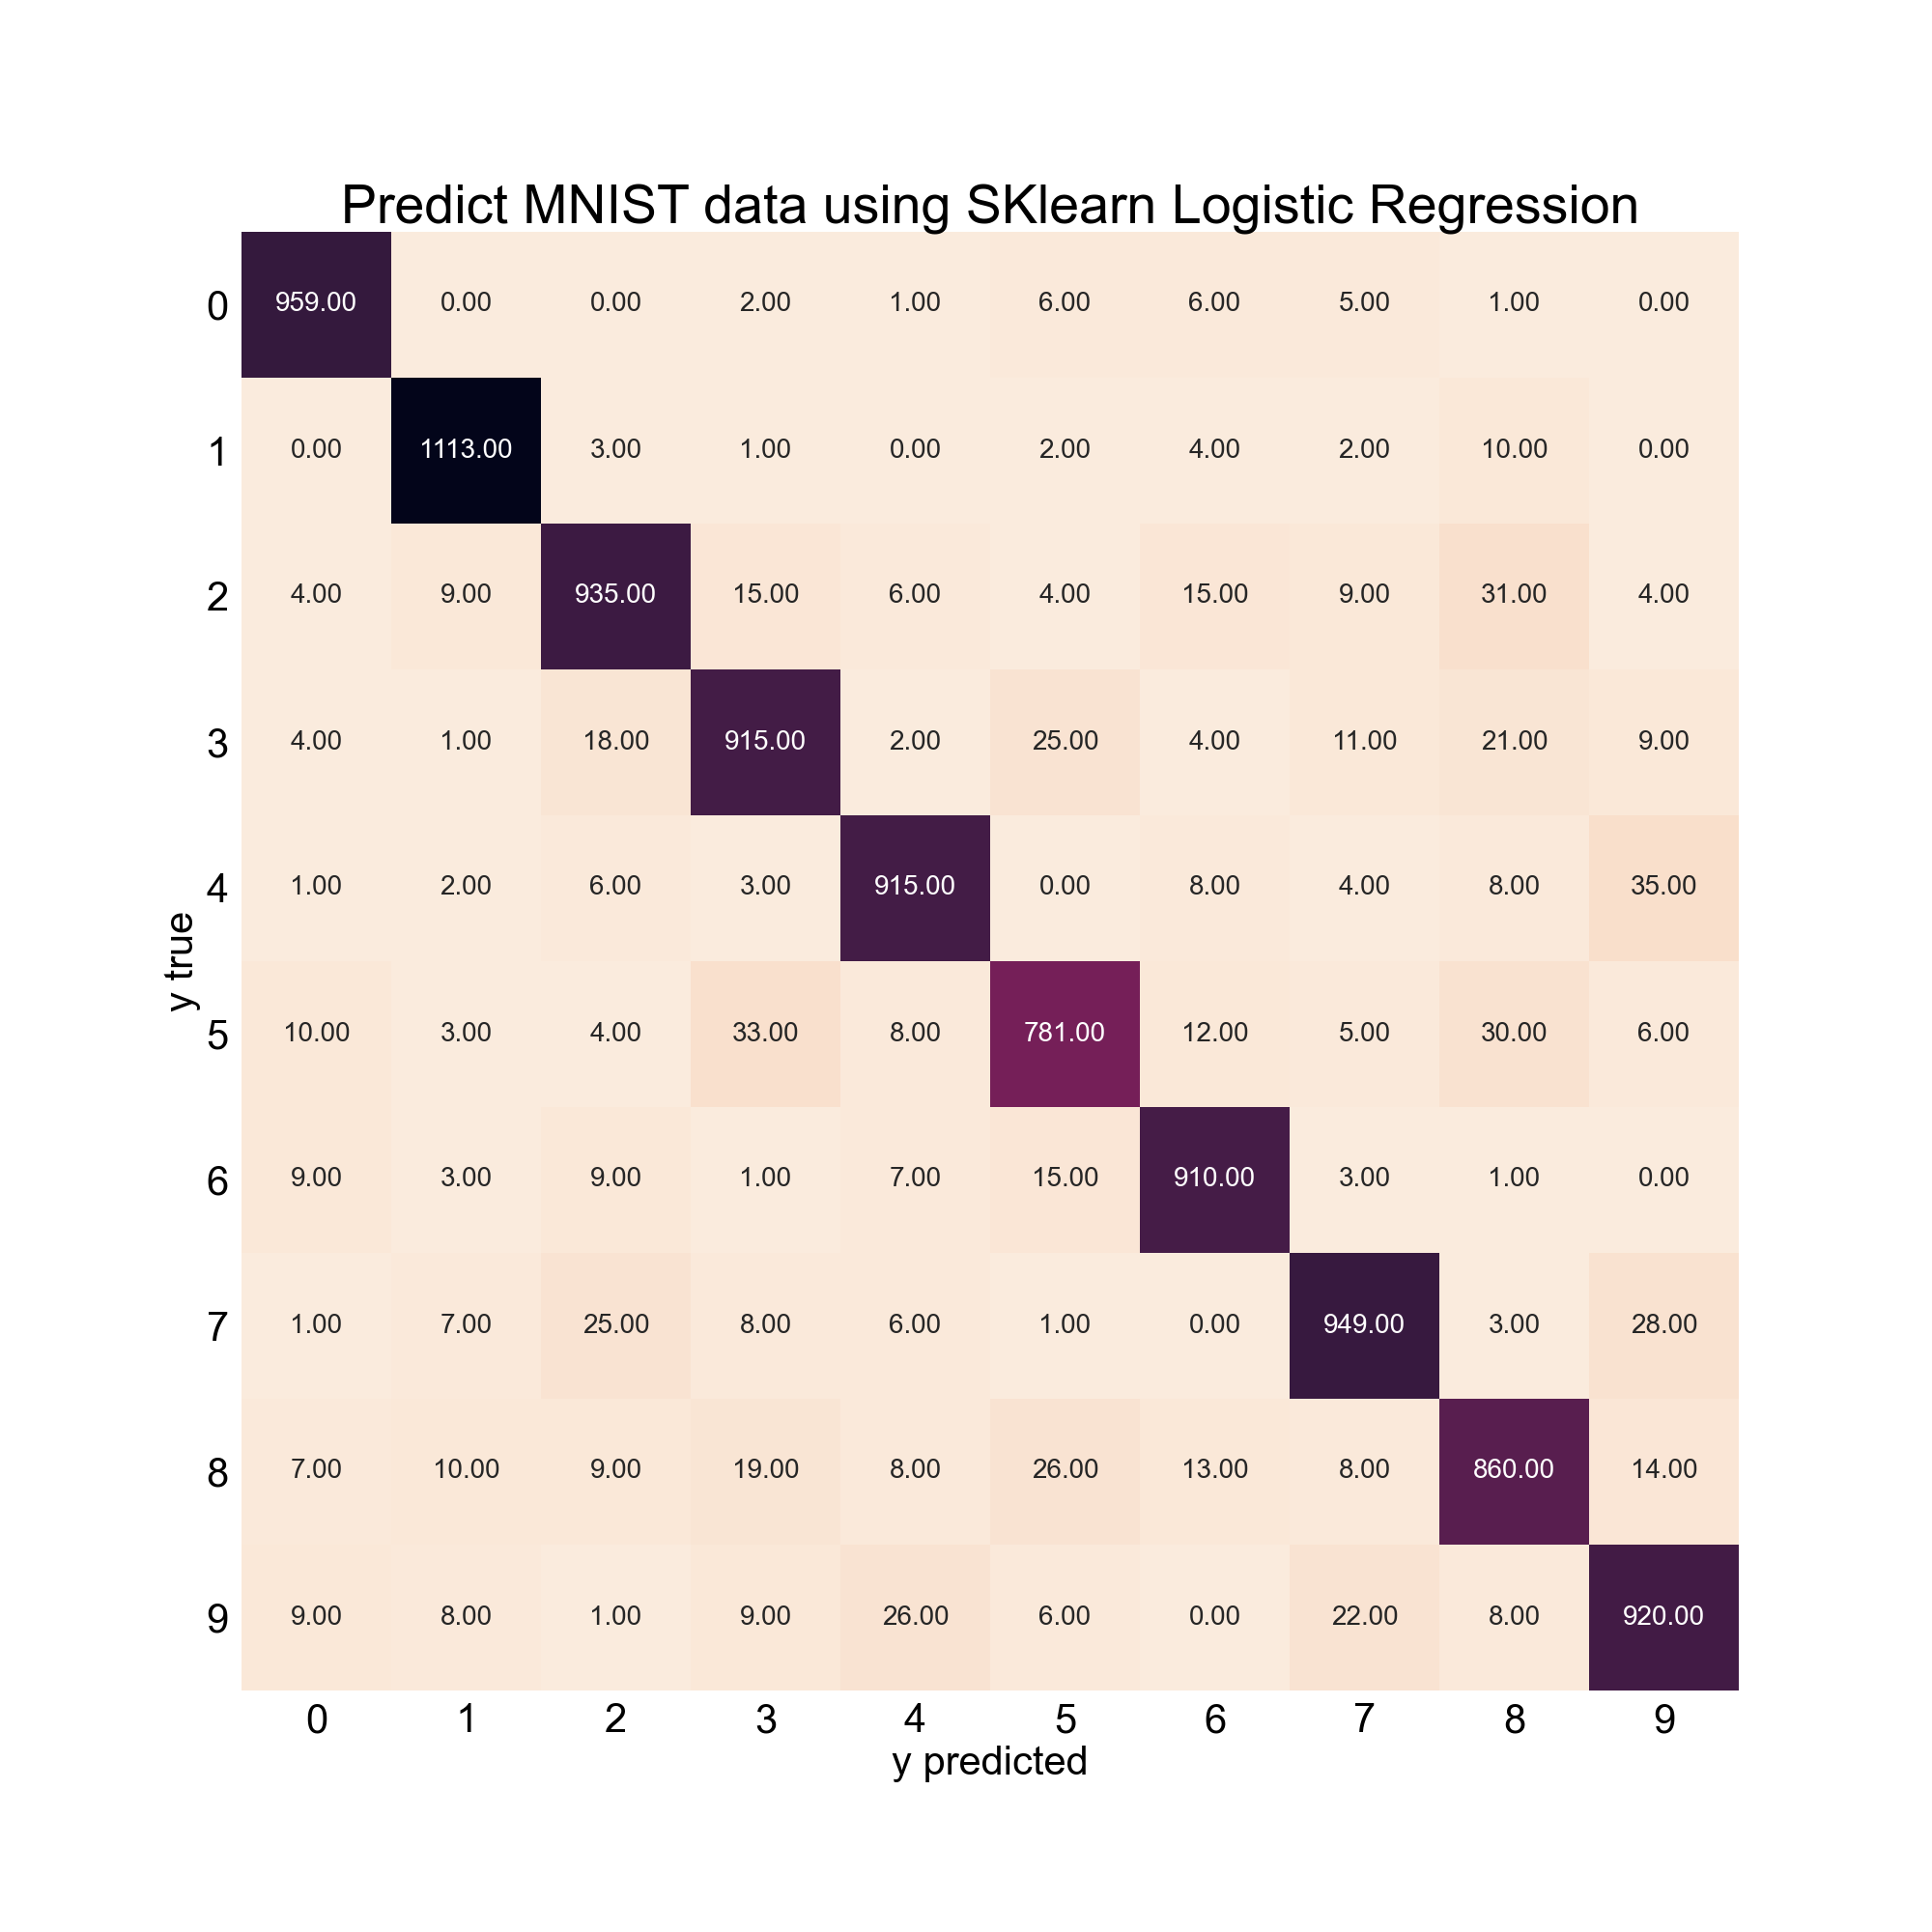
\includegraphics[width=7.9cm]{Figures/MNIST_confMatrix_sklearn_logreg.png}
\caption{Confusion matrix obtained using by training a logistic regression algorithm and apply it on the MNIST test data}
\label{fig:confmatrixlog_MNIST}
\end{figure}

\subsubsection{Classification of ECG-data}
The logistic regression model trained for 1000 iterations on the ECG PTB-XL data set achieved a accuracy score of 0.129 on the test set. The performance on the test set is also shown in figure \ref{fig:confmatrixlog_ecg} as a confusion matrix. 
\begin{figure}[htbp!]
%\centering
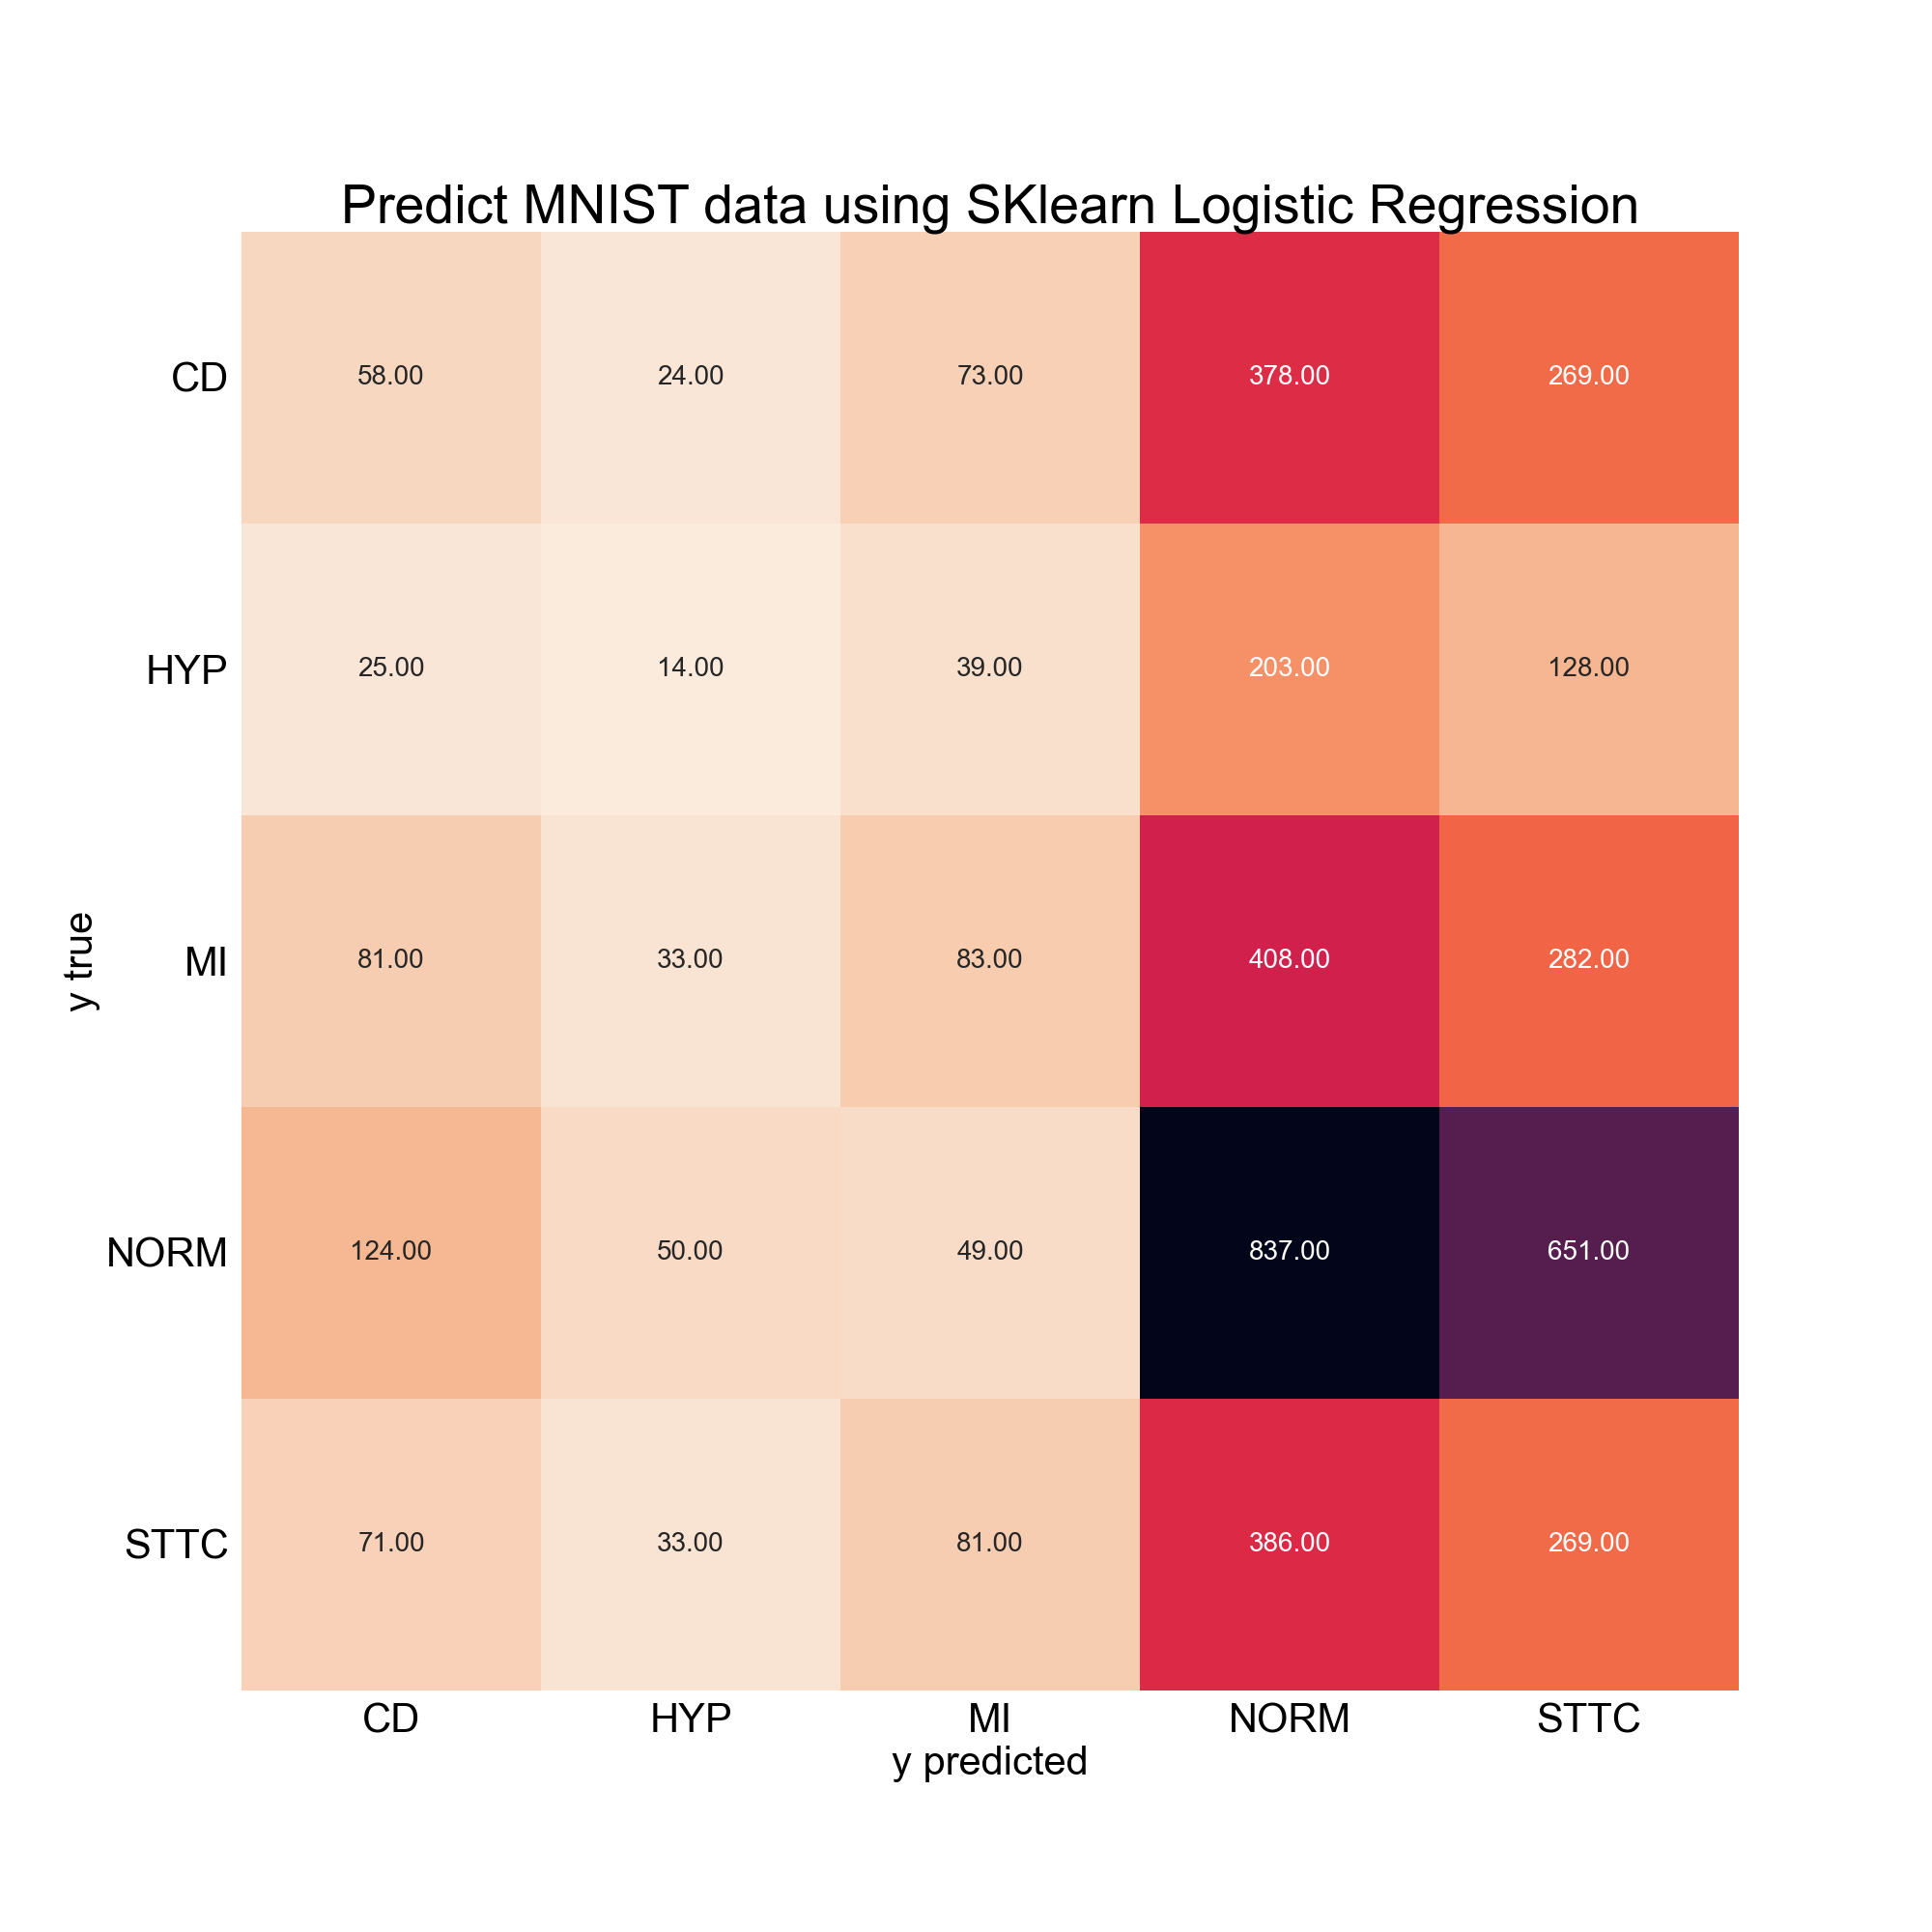
\includegraphics[width=7.9cm]{Figures/ECG_confMatrix_sklearn_logreg.png}
\caption{Confusion Matrix of the result from the Logistic regression function classifying the PTB-XL ECG test data}
\label{fig:confmatrixlog_ecg}
\end{figure}


\section{Discussion}
The normal OLS and Ridge regression models developed in \cite{bjorn-jostein_singstad_using_nodate} were further improved in this study by adding more flexibility. The models were now able to use infinite high order of polynomials. When implementing the SDG optimizer (in the OLS algorithm) the opportunity of adding polynomial features were added. This did not work well and gave R-scores in the order of $10^{-20}$. Thus, the SciKit-learn OLS SGD regression algorithm was used instead but the partial fit method did not work well either.

The regression using neural network was done using TensorFlow \cite{martin_abadi_tensorflow_2015}. This model performed better than the normal OLS and Ridge regression algorithms. But, still it remains unclear how a OLS and Ridge regression with SDG optimzer would have performed compared to these models.  

The classification of the MNIST data was done using a neural network developed from using Numpy \cite{van_der_walt_numpy_2011} and a Logistic regression algorithm from Scikit-Learn \cite{pedregosa_scikit-learn_2011}. The neural network performed a cross-validated accuracy score of $0.851\pm0.002$ and at a test score of 0.866 while the logistic regression outperformed the neural network on the test set with an accuracy score of 0.93, but no cross-validated score was achieved for the logistic regression model. The confusion matrix in figure \ref{fig:NN_mnist_confmatrix} shows that the neural network mainly misinterprets four and nines and threes and fives. This also seems to be the case for the Logistic regression (figure \ref{fig:confmatrixlog_MNIST}). This can also be understandable from a visual point of view.

There have been a few attempts on classifying the ECGs in the PTB-XL database. The classification problem used in this study is called diagnostic superclass. The best result documented on the authors GitHub repository \footnote{\url{https://github.com/helme/ecg_ptbxl_benchmarking#4-ptb-xl-diagnostic-superclasses}} is achieved by a model named resnet1d\_wang which got an AUC score of 0.930 on the proposed test set. Unfortunately there was not obtained any AUC-score from the logistic regression or neural network on the test set. But, during training of the neural network the AUC for training and validation was monitored and varied in the range of 0.6 to 0.7. This indicates that 1D Convolutional neural networks, such as resnet1d\_wang, outperforms simple neural networks and logistic regression in ECG classification. Another possible way to improve the classification would be to use a cluster algorithm like majority voting before the neural network.


\section{Conclusion}
In this study it is shown that a neural network performs slightly better than normal OLS and Ridge regression on data generated by Franke's function when measuring performance in terms of R2-score. 

The logistic regression performed better than the neural network on the MNIST data, but on the ECG data the Neural network performed better than the logistic regression. A possible explanation is that neural networks performs relatively better when the complexity of classification problem increases.

\bibliographystyle{naturemag}
\bibliography{references}
\onecolumn
\appendix
%\section{Appendix}

\begin{figure}[htbp!]
\centering
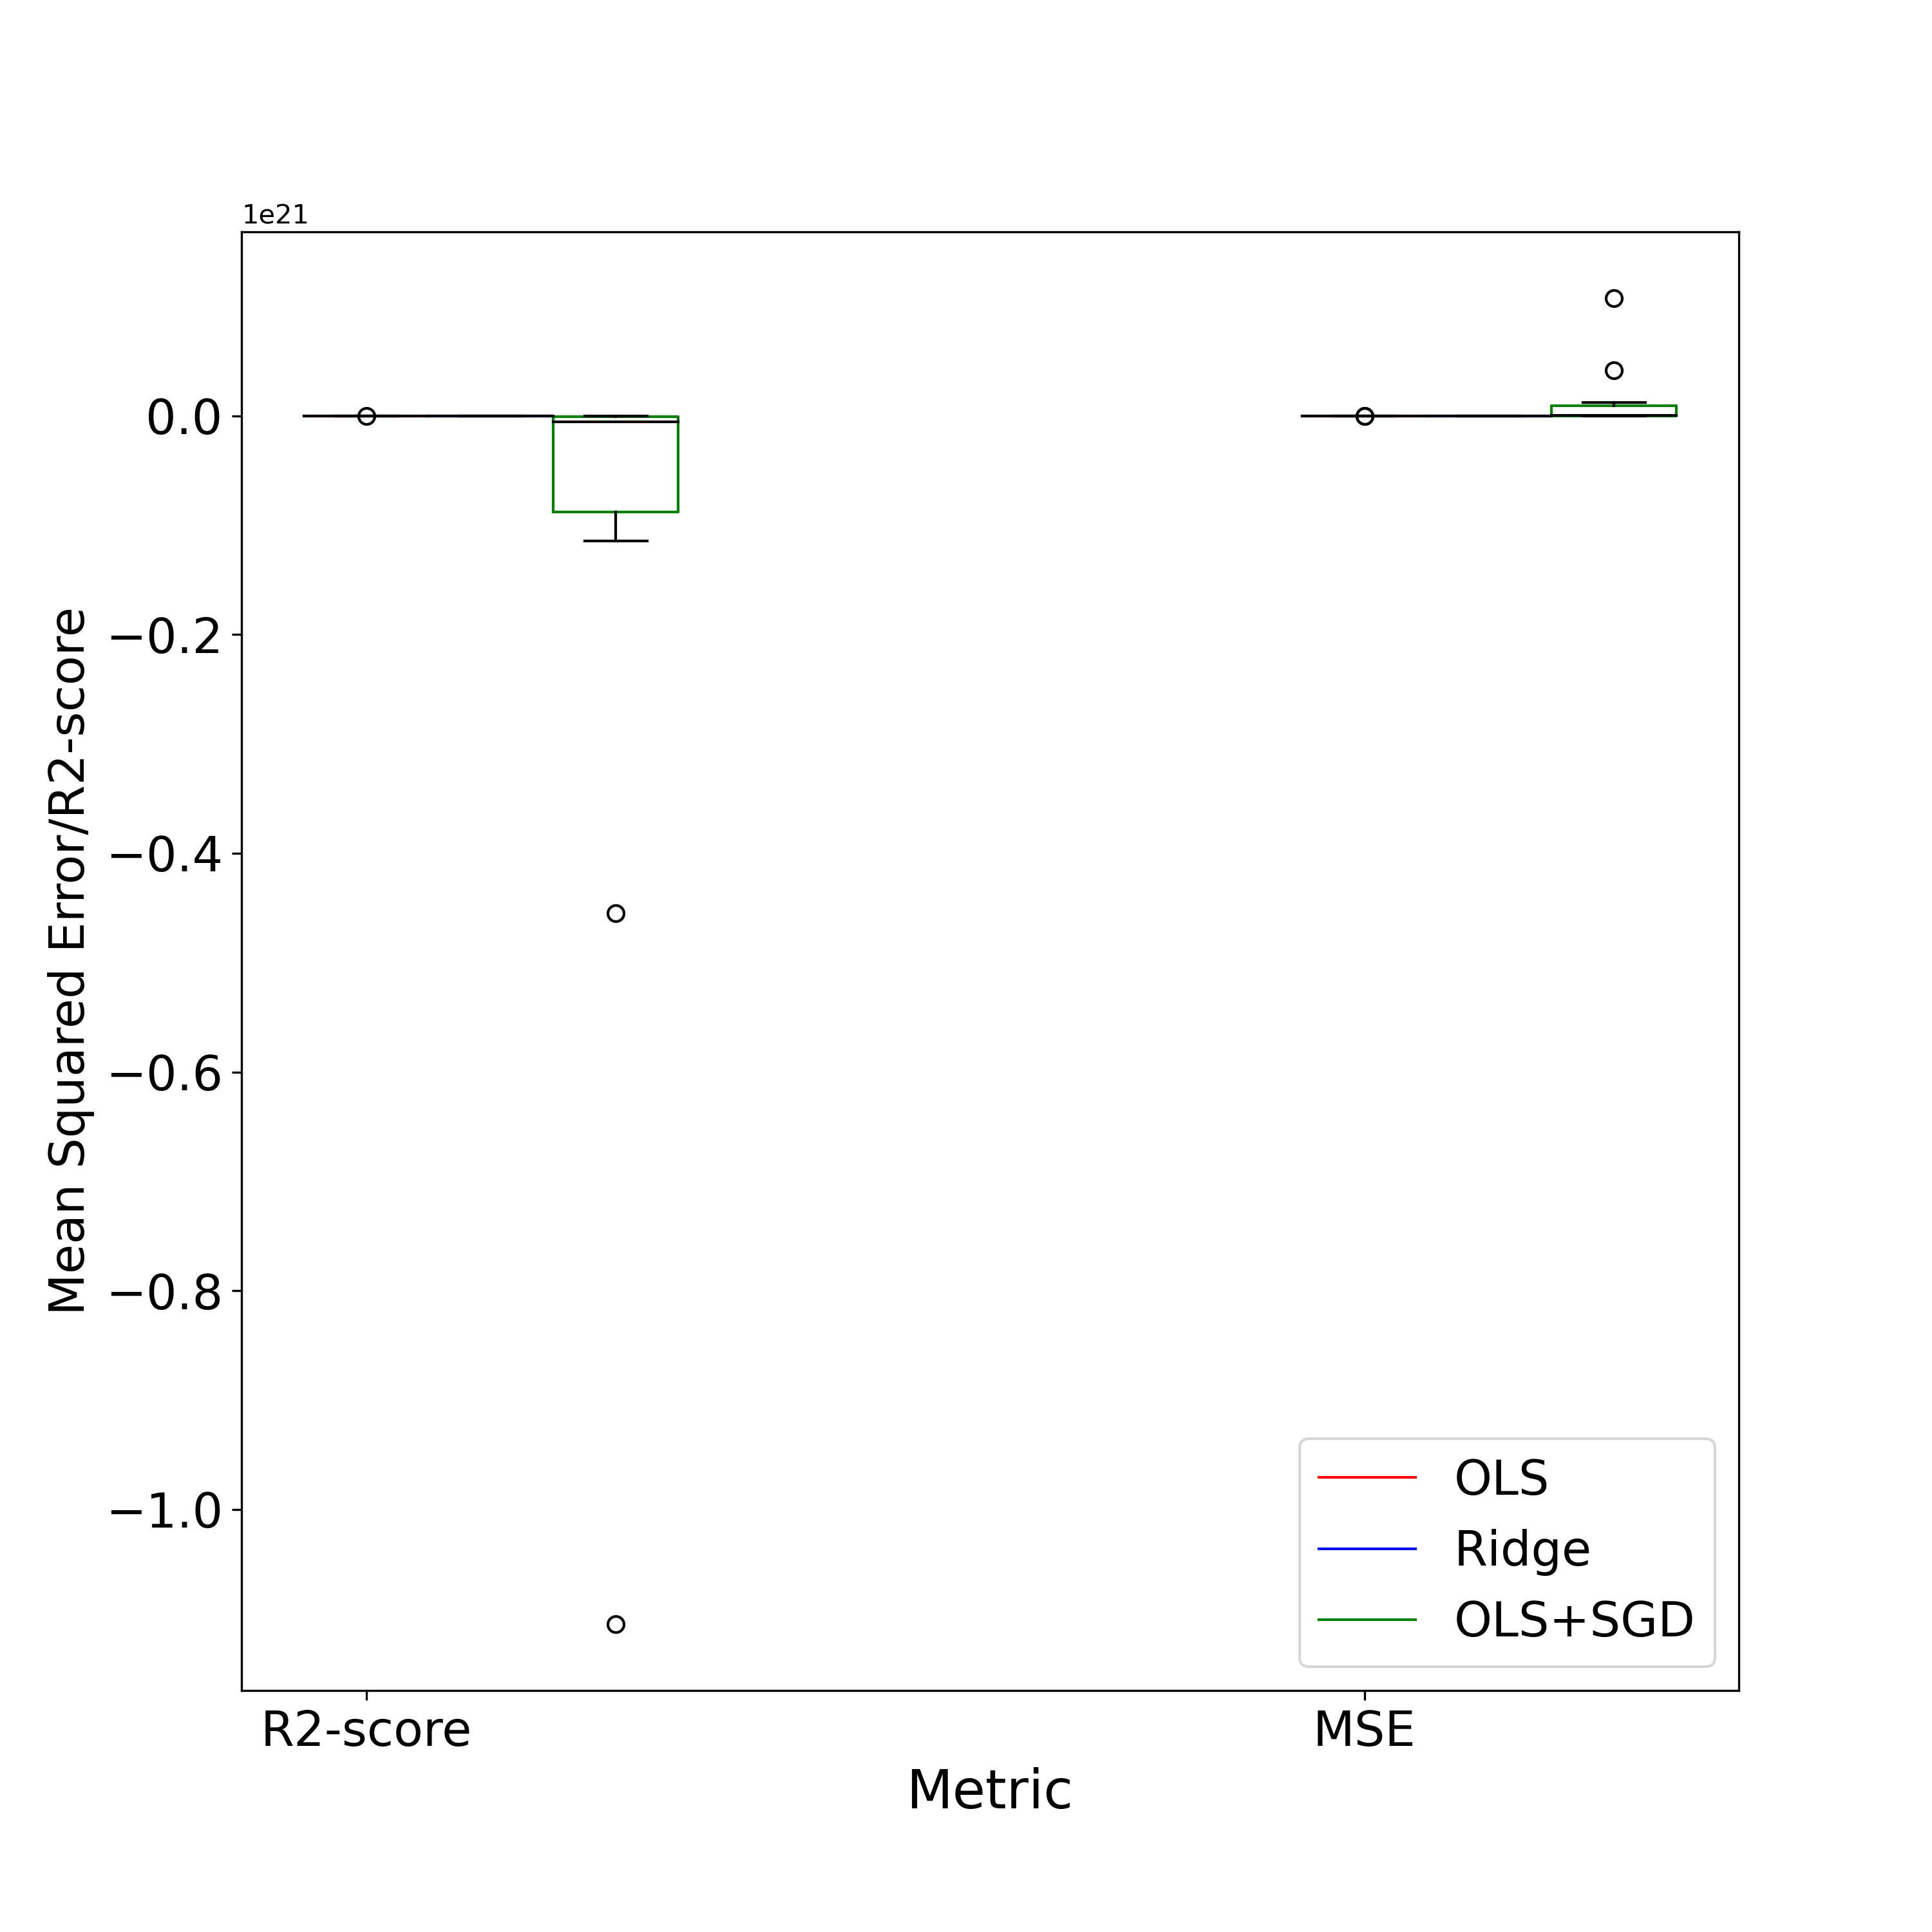
\includegraphics[width=0.65\textwidth]{Figures/boxplot_OLS_ridge_sgd.png}
\caption{R2-score and MSE score for a Ridge,OLS and OLS SGD model}
\label{fig:appendix_sdg}
\end{figure}

\end{document}

